%%%%%%%%%%%%%%%%%%%%% RJT TeX Template %%%%%%%%%%%%%%%%%%%%%
\documentclass[twoside,11pt,a4paper]{article}

%%%% BHAM PREAMBLE - SET THIS FIRST! %%%%
\newcommand{\bhamstudentname}{Zhangda Xu}
\newcommand{\bhamthesistitle}{Thesis Title}
\newcommand{\bhamfronttitle}{Thesis Title Spread\\Over Two Lines}
\newcommand{\bhamschool}{School of Computer Science}
\newcommand{\bhamcollege}{Engineering and Physical Sciences}
\newcommand{\bhamdegree}{MSc. Advanced Computer Science}
\newcommand{\bhamid}{2088192}
\newcommand{\bhamsupervisor}{Dr M. Sridharan}
\newcommand{\bhamyear}{2020}
%%%%           %%%%


\usepackage[hyphens]{url}
\usepackage[breaklinks]{hyperref}
\usepackage{fancyhdr}
\usepackage[sort]{natbib}
\usepackage{comment} % from http://www.latex-community.org/forum/viewtopic.php?f=5&t=4538
\usepackage{dirtree} % from http://blog.plenz.com/2011-07/represent-directory-structures-in-latex.html
\usepackage{longtable} % from http://stackoverflow.com/questions/2896833/how-to-stretch-a-table-over-multiple-pages
\usepackage{algorithm}
\usepackage{algorithmic}   %both algorithm* from http://hasini-gunasinghe.blogspot.co.uk/2014/02/presenting-algorithmsprotocols-in-neat.html

\renewcommand{\algorithmiccomment}[1]{#1} %http://tex.stackexchange.com/q1uestions/61861/algorithmic-package-for-loop-and-comment-at-the-same-line

\pagestyle{fancy}
\renewcommand{\sectionmark}[1]{\markboth{#1}{}}	%from tex.stackexchange.com/questions/111361

\lfoot{\bhamstudentname}
\cfoot{}
\rfoot{}
\fancyhfoffset[L]{0cm} %this fixes the right page number margin issue.
\newcommand{\HRule}{\rule{\linewidth}{0.5mm}}
\renewcommand{\headrulewidth}{0pt}
\newcommand{\tab}{\hspace*{1.25em}}
\newcommand{\minitab}{\hspace*{0.25em}}

%footnote stuff
\usepackage{perpage}
\MakePerPage{footnote} %the perpage package command
\renewcommand*{\thefootnote}{\fnsymbol{footnote}}

\lhead{}\chead{}\rhead{}
\setlength{\headheight}{28pt} %fixes the warnings about headheight being too small
\setlength{\headsep}{6pt}
\pdfoutput=1 % we are running PDFLaTeX
\usepackage[left=2.55cm,right=1.6cm,top=1.8cm,bottom=1.8cm]{geometry}
\usepackage{titling}
\setlength{\droptitle}{-2.75cm}   % This is your set screw\\
\usepackage{titlesec}
\titleformat*{\section}{\normalsize	\bfseries}
\titleformat*{\subsection}{\small \bfseries}
\titleformat*{\subsubsection}{\footnotesize \bfseries}
%modifies the size of the gaps between the top of the title and bottom
% arguments {type}{left}{top}{bottom}
\titlespacing*{\section} {0pt}{3ex plus 1ex minus .2ex}{2ex plus .2ex}
\titlespacing*{\subsection} {0pt}{2.25ex plus 1ex minus .2ex}{0.75ex plus .2ex}
\titlespacing*{\subsubsection}{0pt}{2.ex plus 1ex minus .2ex}{0.5ex plus .2ex}

\setlength{\intextsep}{0pt} %from http://tex.stackexchange.com/questions/25828/how-to-remove-change-the-vertical-spacing-before-and-after-an-algorithm-environ

\usepackage[pdftex]{graphicx}
\usepackage{enumitem}
\usepackage{pdfpages}
\usepackage{lastpage}
\usepackage{amsmath}
\usepackage{amsfonts}
\usepackage{amssymb}


\usepackage{epstopdf} %http://dirkraffel.com/2007/11/19/include-eps-files-in-latex/comment-page-2/

\usepackage{listings}
\lstset{
 basicstyle=\ttfamily,
  columns=fullflexible,
  keepspaces=true,
breaklines=true
} %from http://tex.stackexchange.com/questions/121601/automatically-wrap-the-text-in-verbatim

\newcommand{\todo}[1]{\textcolor{red}{TODO: #1}\PackageWarning{TODO:}{TODO found: #1!}} %from http://tex.stackexchange.com/questions/9796/how-to-add-todo-notes

\DeclareGraphicsExtensions{.jpg}
%%%%%%%%%%%%%%%%%%%%%  END of TEMPLATE %%%%%%%%%%%%%%%%%%%%%

\title{MSc. Project\\\bhamthesistitle}
\author{\textsf{\bhamstudentname {\textsf{Degree Postnomials}}}}

\date{}
\begin{document}

\pagenumbering{gobble} % fix at	 http://tex.stackexchange.com/questions/7355/how-to-suppress-page-number
% this came from http://en.wikibooks.org/wiki/LaTeX/Title_Creation and http://tex.stackexchange.com/questions/14778/error-with-hrule
\begin{titlepage}
\begin{center}
% this was from http://tex.stackexchange.com/questions/7219/how-to-vertically-center-two-images-next-to-each-other
\begin{minipage}{6in}
  \centering
  \raisebox{-0.5\height}{
\includegraphics[width=1.25in]{crest}}
  \hspace*{.2in}
  \raisebox{-0.5\height}{
\includegraphics[height=0.9375in]{uni}}
  \end{minipage}
  \\ [1.0cm]
\textsc{{\LARGE \bhamschool\\}College of \bhamcollege}\\[3.5cm]

\textsc{\Large MSc. Project}\\[0.5cm]

% Title
\HRule \\[0.4cm]
\begin{center}\Huge
\bhamfronttitle
\end{center}
\HRule \\[1.5cm]
% Team and Members

\begin{center}
Submitted in conformity with the requirements\\ for the degree of \bhamdegree\\
\bhamschool\\ University of Birmingham\\
\vspace{2cm}
\bhamstudentname, BSc. (Hons)\\
Student ID: \bhamid\\
Supervisor: \bhamsupervisor
\end{center}
\vfill

% Bottom of the page
{\large September \bhamyear}

\end{center}
\end{titlepage}

\section*{Declaration}
% Taken from the MSc Thesis template, and edited for a PGT report
The material contained within this report has not previously been
submitted for a degree at the University of Birmingham or any other university.
The research reported within this report has been conducted by the author
unless indicated otherwise.\\


Signed ..........................................................................................................................................
\vfill
\clearpage
\begin{center}
\vspace*{\fill}
\begin{minipage}{6in}

%\centering \Large{``Most men who have really lived have had, in some share, their great adventure.\\This railway is mine."}\\{\normalsize{\textsc{James J. Hill}}, \emph{Railway Pioneer}} \vspace{2cm}

%\centering \Large{``Steam engines don't answer back.\\ You can belt them with a hammer and they say nowt."}\\{\normalsize{\textsc{Fred Dibnah}}, \emph{Steeplejack and Engineer}} \vspace{2cm}

\centering \Large{``You have to learn the rules of the game.\\ And then you have to play better than anyone else"}\\{\normalsize{\textsc{Albert Einstein}}}

  \end{minipage}
  \vspace*{\fill}
\end{center}


\clearpage
\maketitle
\vspace{-5.5em} %fixes distance between \maketitle and the TOC
\begingroup
    \fontsize{9pt}{11pt}\selectfont
\tableofcontents
\endgroup
\clearpage
\phantomsection
\section*{Table of Abbreviations}
\begin{itemize}[nolistsep]
\item 3DES -- Triple DES
\item 3G -- Third Generation
\item AES -- Advanced Encryption Standard
\item ALE -- Adaptation Layer Entity
\item API -- Application Programming Interface
\item ATOC -- Association of Train Operating Companies
\item ATP -- Automatic Train Protection
\item CAN -- Controller Area Network
\item CBC-MAC -- Cipher Block Chaining Message Authentication Code
\item CBTC -- Communication Based Train Control
\item CFM -- Communication Functional Module
\item CRC -- Cyclic Redundancy Check
\item CSR -- Cab Secure Radio
\item CTRL -- Channel Tunnel Rail Link
\item (D)DOS -- (Distributed) Denial of Service attack
\item DES -- Data Encryption Standard
\item DMI -- Driver Machine Interface
\item EDE -- Encrypt-Decrypt-Encrypt
\item EED -- Encrypt-Encrypt-Decrypt
\item EFF -- Electronic Frontier Foundation
\item EIRENE -- European Integrated Railway Radio Enhanced Network
\item ERA -- European Rail Agency
\item ERTMS -- European Rail Traffic Management System
\item ETCS -- European Train Control System
\item EVC -- European Vital Computer
\item GPRS -- General Packet Radio Service
\item GSM -- Global System for Mobile Communications
\item GSM-R -- Global System for Mobile Communications for Railway
\item HMAC -- Hash-based Message Authentication Code
\item HS1 -- High Speed 1
\item HTTP(S) -- Hypertext Transfer Protocol (Secure)
\item IP -- Internet Protocol
\item IV -- Initialisation Vector
\item KMAC -- Key used as a seeding key to generate the Session Key, KSMAC
\item KMC -- Key Management Centre
\item KMS -- Key Management System
\item KSMAC -- Session Key used for MAC calculations
\item KVB -- Contr\^ole de Vitesse par Balises (Speed Control by Beacons)
\item LEU -- Lineside Electronic Unit
\item LRBG -- Last Relevant Balise Group
\item LTE -- Long Term Evolution
\item LZB -- Linienzugbeeinflussung (Continuous Train Control)
\item MA -- Movement Authority
\item MAC -- Message Authentication Code
\item MORANE -- Mobile Radio for Railways Networks in Europe
\item NRN -- National Rail Network
\item OBU -- On-Board Unit
\item PZB -- Punktf\"ormige Zugbeeinflussung (Intermittent Train Protection used in Germany)
\item RAIB -- Rail Accident Investigation Branch
\item RBC -- Radio Block Centre
\item RETB -- Radio Electronic Token Block
\item RIU -- Radio Infill Unit
\item RSG -- Reliability Steering Group, part of RSSB
\item RSSB -- Rail Safety and Standards Board
\item SAI -- Safe Application Interface
\item SaPDU -- Safety Protocol Data Unit
\item SCADA -- Supervisory Control and Data Acquisition
\item SCEPTICS -- SystematiC Evaluation Process for Threats to Industrial Control Systems
\item SFM -- Safety Functional Module
\item TCP -- Transmission Control Protocol
\item TPM -- Trusted Platform Module
\item TTT -- Triple Time Stamping
\item TVM -- Transmission Voie-Machine
\item UIC -- Union Internationale de Chemins de Fer
\item UNIFE -- Union des Industries Ferroviaires Europ\'eennes
\item UNISIG -- Union Industry of Signalling
\end{itemize}

\textit{Note to the user of this template. I highly recommend using the \texttt{acronym} package, as follows.}
\begin{verbatim}
1. Place the following in the preamble of this document:
\usepackage[printonlyused]{acronym}  % this will build the acronym list
                                     % on the fly from a source file called `acronyms.tex'
2. In acronym.tex, define the acronyms (see the instructions in the included file)
3. Place the following TeX code where you want the acronyms to be displayed:
\input{acryonyms}
4. Usage of the acronym package is as follows:
\acf{ABC} will put in the full version of the acronym for ABC. If you want to
refer to an acronym, but don't want to use it's full expansion, use \ac{ABC}.
Plurals can be done, e.g. \acfp{ABC}. LaTeX isn't smart with plurals, so see the
overrides given at
http://anorien.csc.warwick.ac.uk/mirrors/CTAN/macros/latex/contrib/acronym/acronym.pdf

\end{verbatim}

\addcontentsline{toc}{section}{Table of Abbreviations}
\clearpage
% set up the page numbering and counter - Table of Abbreviations has no page number
% also set up the footers and headers appropriately.
\pagenumbering{arabic}
\setcounter{page}{1}
\lhead{}\chead{MSc. Project Report :: \nouppercase{Section \thesection\minitab :: \leftmark}}\rhead{}
\rfoot{Page \thepage \hspace*{0.2pt} of \pageref{LastPage}}
\renewcommand{\headrulewidth}{0.4pt}

\section{Overview}
This paper is a formal analysis of the communication protocols and standards which are used as part of the European Rail Traffic Management System (ERTMS) platform. This report has a particular focus on identifying key components of GSM-R in the context of ERTMS, identifying areas of vulnerability and exposure, and proposing potential solutions for improvement.

\subsection{Abstract}
The UK Rail Network handled some ``1.6 billion journeys ... travelling over 37 billion miles" during 2013-14 \citep{RailExecutive14a}. At present, the UK rail network is reliant on existing infrastructure that dates back to the 1960s \citep{NetworkRail12a}, where signalling is provided through line-side equipment, which relays aspects to the train driver. This, in turn, is interpreted either as a `Movement Authority' (MA) which gives permission to proceed into the next `block'\footnote{A `block', in railway terminology, is a stretch of track on any given line.} or alternatively an order to stop, should another train occupy the block ahead. One issue with this system is reliability. As the signals are line-side, cable and system failures lead to delays, which impact day-to-day operations.

The current platform for UK rail signalling does not provide an opportunity for necessary growth, as passenger volumes increase, and the need for a human to interpret and react to signals detracts from the potential capacity and speed of a given line. One such example is the West Coast Main Line, where Railtrack, the then-predecessor to Network Rail planned to implement Moving Block signalling, providing line-speeds of up to 140mph. However, due to issues encountered during the project, the existing (unchanged) system was retained, leading to line-speeds being restricted to 125mph. In contrast, in 2015, the Channel Tunnel Rail Link (CTRL/HS1) has line speeds of between 230km/h (approx. 143mph) and 300km/h (approx. 186mph)\citep{RailTech15} -- a considerable increase, due to the use of the TVM and KVB systems, which are cab-based systems, providing signalling and speed information directly to the cab. This, however, has issues with inter-operability where a number of systems are required to operate a train in different countries \citep{IRJ14a}.

The solution for these capacity issues, whilst also improving safety and reliability, is ERTMS. This platform, which has four levels of operation, discussed in this report, transforms a line-side signalling system and creates it into a network capable of a `moving block' system at the highest level. At the core of this system is GSM-R, a rail implementation of the GSM Standard, providing a means for signalling and other line information to flow between the train and the network. This will be reviewed later in this paper. ERTMS also provides a platform for common signalling, allowing rail vehicles to transit between countries seamlessly without the need to switch to a different signalling system, reducing the opportunity for human error.

Whilst ERTMS is largely standardised, it relies on an otherwise open communications channel (GSM) for data-flow. The use of GSM-R within ERTMS adds the provision of a `safety layer', EuroRadio, and other rail-specific applications. The core focus of this project was to analyse these layers and determine if they provide a secure and trusted medium for communications between ERTMS entities. Through formal analysis of train to trackside communications in ERTMS, potential vulnerabilities were exposed and recommendations made to improve the security of the platform.

\subsection{Acknowledgements}
The culmination and success of this project would not have been possible without the kind help, wisdom and support of many people, some of whom deserve special mention.

To my Project Supervisor, Tom Chothia, and Joeri de Ruiter for our numerous meetings discussing and mapping extensive specification documents, furthering our understanding of ERTMS and ultimately shaping this project, delivering new concepts to investigate as part of ongoing research.

To my friends, who have listened to the countless ideas to improve security, to make this project unique in many ways, with the hope it will one day make a difference to commuters and rail bodies.

To my family, spending endless hours proof-reading, reading up and following the progression of ERTMS adoption to ensure I did not miss anything during this project. Their patience has been fantastic, and their help is greatly appreciated.

% Grandparents

\clearpage
\section{Introduction}
The aim of this project was originally to assess three components which contribute to form ERTMS: GSM-R, Eurobalises and the Vehicle Area Network. Within this, I would assess specifications for these components and establish vulnerabilities which may be exploited by an attacker and determine potential areas for improvement. That said, GSM-R is one of the most important elements which forms ERTMS, as the critical `umbilical cord' used by ERTMS entities, not only track-side but also onboard the train. The decision was therefore taken to focus specifically on GSM-R and those elements which are an enhancement to the everyday GSM protocol.

During my time at the University of Birmingham, I have experienced the frustration of train delays, frequently due to line-side equipment or signalling failure. When I was invited to work on the SCEPTICS Project, it became clear from discussions that, with the introduction of ERTMS, which removes infrastructure which commonly fails, these problems would be minimised. Where possible, areas of failure would then be primarily restricted to the train and underlying communication infrastructure. During 2013/14, the public performance measure (PPM) was rated at 90.0\%, where 10\% of trains were more than 5\footnote{For regional, London and South-East services} or 10\footnote{Long-distance services} minutes late. The passenger satisfaction survey for that year had punctuality, reliability, speed and frequency as the most common complaints \citep[p. 3]{RailExecutive14a}.

ERTMS offers significant improvements for rail travel, providing a common infrastructure for rail vehicles to use and provide a real-time communication interface between the train and signalling centre. This, however, means that both the specification and implementation must be robust and fit for purpose. It is this area which inspired part of the project, where cyber-security relies on strong specifications and implementations to prevent any attacks taking place, which could have a number of impacts, from `minor' incidents such as train delays, to a scenario with potentially fatal consequences.

Rail has been a way to drive industry and travel, with some goods travelling up to 11,000km at a speed twice of that compared to sea, whilst being ``one of the greenest means ... on the market"\citep{EuropeanCommission13a}. Trains are getting `smarter' with many manufacturers ``increasingly moving to manufacturer-specific ... platforms with proprietary train control systems, ..., thus the trend in recent years has been away from interoperability"\citep[pp. 13]{DfT15a}. This shift means that the underlying systems also cannot be scrutinised, given the closed nature of code and infrastructure. Even if the ERTMS platform could be  proven to be safe, secure and immune to a majority of threats, flaws in vendor-specific systems could still compromise this foundation.

Digitising systems in any industry, especially industrial control systems, means that attack vectors which were not previously possible may now be attainable and, given that ERTMS is still considered to be relatively new and emerging, it requires close scrutiny to ensure it is both safe and secure, not only from `script kiddies' but also sophisticated attackers.

Industrial control systems are critical, supplying power, transport and other key supplies for everyday life. Recent attacks have taken place on these systems, including Stuxnet, Duqu and Flame, in addition to other attacks on SCADA and alternative industrial control systems, for example aviation. Attacks on these systems present a potentially significant threat, therefore, to everyday life.

With ERTMS, a next-generation digital solution, if adequate cyber-security practices have not been implemented, an attacker is able to render a parameter of an underlying system incorrect or modify it by unauthorised means. As identified above, the GSM-R communication link between train and track is the `umbilical cord' for ERTMS. If this link was compromised, the security and safety of the train and its passengers could be jeopardised. The research conducted and reported in this paper therefore assesses and recommends improvements to the integrity of ERTMS to deliver a safer, more reliable and secure platform for the future. The UK Government plans to introduce ERTMS/ETCS Level 2 on 72\% of the rail network by 2044. It is critical, therefore, to ensure that it is a safer and more secure alternative to the platform it is replacing. A formal analysis of this platform would be required by the security community to ensure that these specifications, agreed and ratified by committee, provide a sustainable and secure platform, compared to other specifications like EMV which have vulnerabilities through the way they were formally ratified.

As Peter Gibbons, Head of Cyber-Security at Network Rail appropriately says, ``we need to stop looking at cyber security workers as magical people and help the train drivers and oil workers to see an issue and respond to it, viewing security as a part of their job and calling in the expertise when they need it"\citep{V315a}. Major standards, whether they are for industrial control systems or motor vehicles, should be designed and then formally modelled and analysed to ensure that both meet the required specifications and do not introduce any additional attack vectors. With vendors bidding for ERTMS deployments around the world, their proprietary systems communicate with the ERTMS platform, but are not entirely open, per se. Closed systems may hide potentially serious vulnerabilities which could compromise not only one train but many.

Network Rail in 2014 \citep{Computerworld14} acknowledged that a move from a ``relatively Victorian" system to a digital solution ``opened up a new risk, and for [Network Rail] that is cyber risk". In 2013, a cyber-security strategy was published, identifying cyber security ``a key priority" \citep{NetworkRail13a}, however their attitude to risk is in stark contrast to what security researchers would have expected. If a threat was found, and it would not be immediately exploitable, then ``we will not commit resources to mitigate risks". For such a large system as ERTMS, if resources were not allocated to resolve the weaknesses and vulnerabilities identified in this paper with immediate effect, then by the time the patches were published and included in an ERTMS version, it could be too late. The risk of taking such an approach is that threats may materialise sooner than predicted, as the computational power of computers becomes greater and as new tools are published, which would allow an attacker to get closer to their end-goal more quickly.

That said, it is critical when weighing up the relative risk of such attacks taking place, to consider the implementation cost of the appropriate changes to defend against them as these changes may be uneconomic. There must, therefore, be a balance between risk and exposure to vulnerabilities, where the financial cost to patch a vulnerability may be \pounds150,000 per rail vehicle, which may be considered uneconomic, compared to a physical attacker who puts a sleeper on the train line to achieve the same outcome.

The research presented in this project paper comes from reading, reviewing and modelling the various specifications from which ERTMS is composed, taking it from its low-level origins and establishing links between each component and assessing how dataflow is established between components. Protocols would then be analysed in depth using formal verification tools including Proverif to determine whether those elements are secure or not. If they were deemed insecure, or not considered sufficiently secure for the future, the impact would be propagated to `users' of that element, to assess how far that vulnerability could succeed without detection.

This paper examines, determines and highlights the security of train and trackside communication used in ERTMS. Through formal analysis of individual protocols and constituent elements, areas vulnerable to attack are identified with potential solutions proposed which would not only assist ERTMS in increasing capacity, but also improve the overall safety and security of the rail network.\\\\\\

\begin{center}
``Strive for perfection in everything you do. Take the best that exists and make it better.\\When it does not exist, design it."\\-- Sir Henry Royce

\end{center}

\clearpage

\section{The Current UK Rail Signalling Platform}
\subsection{Overview}
At present, with the exception of the Great Western line, running from London to Wales, the UK heavy-rail network is largely standardised allowing a number of vehicles, whether it be freight or passenger trains, to operate on the same track. What makes the Great Western line different to the rest of the UK network is the deployment of Automatic Train Protection (ATP), an advanced system which supervises the train to ensure it does not pass a line-side signal at danger or travel at a speed higher than that which is permissible on the line \citep{BBCATP00}. This system was introduced following the Hatfield rail accident, which resulted in four fatalities and seventy casualties. Elsewhere on the network, a simpler system is used to ensure safe running of the railway, which implements line-side signals and balises to protect lines by indicating if the signal ahead shows if the line is clear.

Commonly, signalling takes the form of blocks, with a stretch of a rail line split into these blocks. A train cannot enter a block already occupied by another train, with the precondition that a train should be able to stop before overrunning into the next block when being given a warning aspect. These blocks are of variable length and, depending on a number of factors, such as location (near a station, or major junction), line speed and other operational considerations. A number of components are used to provide signalling in the UK, whilst some other countries already employ wholly digital solutions, with France using TVM and Germany using PZB/LZB.

\subsection{Components}
As mentioned above, a number of components are used as part of the UK rail network to provide the signalling platform. These components are connected together, forming a network to provide a fully managed and safe operational transport system.
\subsubsection{Line-side Signals}
Line-side signals operate in a similar way to traffic lights on public highways and use the same principle for indicating permission to move, where red indicates stop, yellow indicates warning aspects and green indicates that the line ahead is clear.\\
Signals are typically located line-side or mounted on gantries to provide `aspects' to the train driver, indicating permission to proceed into the next supervised block. In `hubs' such as Birmingham New Street, or London Euston, signalling may use four-aspect signals, however, these signals can also relay information including journey routing to the driver. An example of such use would be on approach to a major station, where the route `indicator' highlights the platform at which the train will arrive, or the line to which it will be routed, if used for departure. In other areas of rail lines, triple, double or even single aspect signals may be seen, with possible aspects shown below. Other indicators are also included, however, these are outside the scope of this paper.
\begin{center}
 \includegraphics[scale=.7]{Signals.eps}\\
Figure 3.1: \textit{Example four-aspect signals in use on the UK Rail Network, counting down to a `danger' aspect}
\end{center}

All signals of this type are connected by cable to a line-side cab, which receives information from a central control centre or signalling box\footnote{Network Rail are removing Signal Boxes in favour of signalling centres to use centralised operation centres \citep{GlobalRailNews11a}.}, specifying what aspect to display. Faults may also be automatically detected by these cabs and reported to the appropriate centre for investigation. Signals are uniquely identifiable for this purpose such that in the event of signal failure, the driver of a stranded train may use the signal marker as a location reference.

\subsubsection{Occupancy Detection}
Once a train has successfully moved into the next block, it is considered to occupy this block and not the block beforehand. Information about track occupation can be retrieved through a number of methods.\\Track Circuit detection is one method, whereby an electrical signal is passed through one rail, and, due to the metallic composition of train wheels and axles, they are able to convey current and these signals to the other rail. This signal is picked up by a relay located on the track to identify this occupation. It does not, however, indicate where in relation to the relay the train is located, rather it indicates a positive or negative response.

Another method to identify whether a track is occupied is established through the use of axle counters. These devices are attached to a rail, and count the number of axles passing over them. The concept behind axle counters is that when a train moves into a new managed block, the number of axles that enter the block are counted in, and upon exiting this block, they are counted out. If the number of axles counted in $\equiv$ the number of axles counted out, then the block is considered to be no longer occupied and another train may safely enter it. Track Circuit devices are simply a means of confirming that a block is occupied or not, and are complimentary to axle counters.
\subsubsection{Communications}
Maintaining a communications link between train and trackside is safety-critical to ensure a driver is advised of an issue on the line, or to report issues to signallers, so that appropriate action can be taken.

In the UK, GSM-R has been deployed by Network Rail as part of a project to replace the ageing `National Rail Network' (NRN) with a proven system that offers capacity growth. GSM-R uses the same technology as GSM, which was the basis for mobile communications until recently, before 3G and LTE had gained traction in the sector. Using GSM as a base communications system, GSM-R was ratified for use following the success of the EIRENE Project, conducted by Union Internationale de Chemins de Fer (UIC), the International Union of Railways.

Between 2009 and 2014, Network Rail, the Infrastructure Manager for the UK railway network, completed a nationwide rollout of GSM-R, providing an end-to-end voice service for voice applications, the ability to send and receive pre-defined text messages, and allow group calling. The Cambrian Line, as an extension, with its implementation of ERTMS, also has the additional capability of using GSM-R for Data.

The Cambrian Line utilises not only GSM-R Voice, but also a data standard of GSM-R, to receive signalling and line information. This is achieved via a data modem providing a circuit-switched connection, allowing a constant connection to be held with train operating speeds of up to 500km/h \citep{ClearCinCom09}.

\subsubsection{Interlocking}
Interlocking systems form a critical part of the signalling system, receiving ``requests from the signaller...and executes only if safe to do so" \citep{RailEngineer13a}. The Interlocking systems control the setting and releasing of signals and points to ``prevent an unsafe condition...arising during the passage of trains" \citep{RSSB14a}. When used in ERTMS/ETCS Level 1, a Lineside Electronic Unit (LEU) ``interfaces the ... interlocking equipment with Eurobalise and Euroloop" \citep[p. 15]{SUBSET-044} which provides Movement Authorities directly to the train.

Interlocking systems ensure that ``trains share the network safely" \citep[pp. 10]{NetworkRail15a}. Whilst this system would not have prevented accidents such as Hatfield\footnote{In this case, the driver of the train proceeded through a stop signal.} and Madrid\footnote{This occurred due to an overspeed condition, not through  signalling error.}, it has improved safety by ensuring that no decision can be made to allow a train to enter an occupied section, or modifying routing whilst a section is occupied. This significantly reduced the risk of operating trains, through the incorporation of a fail-safe mechanism.

\subsection{Issues}
The current UK Signalling and Rail Management system is outdated and lags behind some of the available modern solutions used internationally. With age comes increasing reliability and maintenance overhead costs. Clearly, what was deemed a revolutionary solution in the 1960s does not fit with the requirements and needs of today.
\subsubsection{Opportunity for Growth}
The current UK system does not provide a platform for necessary growth in terms of speed and capacity. One such example is the West Coast Main Line, which is one of the busiest \citep[pp. 2]{Parliament10a} rail lines in Europe. Whilst this relies on ageing infrastructure \citep{NetworkRail09a}, signalling is also a key factor restricting capacity. The reliance of drivers to be able to read signals at speed and react appropriately reduces the possible speed at which trains may operate, impacting the number of rail vehicles allowed on a line at any given time. Whilst some lines cannot support higher line-speeds, either due to gradients, curves or line conditions, main lines should be able to allow greater flexibility and provide the opportunity for improved capacity as required.

At present, due to capacity constraints, trains may `chase signals', where they run at a slower speed than the indicated line speed, in anticipation of approaching a danger signal. This leads to consequential delays which further frustrate passengers and puts future services at risk of also being delayed or cancelled.

\subsubsection{Infrastructure Failure}
Signal failure is a common occurrence in the UK. Network Rail performance measures indicate that, on average, 26\% of delays nationally are due to these failures, and that nationally, trains are typically delayed by 2.5 minutes \citep{NetworkRail15e}. The impact of a single delay leads to a snowball effect, with knock-on delays, cancellations and frustration for passengers. One of the main causes of failure is cable theft or damage. Whilst measures have been taken by Network Rail to minimise this type of theft and damage, using products such as Smartwater \citep{SmartWater15a}, this is only a short-term fix to a long term problem. Removing this infrastructure altogether would reduce cost, and improve the reliability of the railway, given there are fewer exposed components.

\subsubsection{Maintenance}
Equipment and infrastructure ages and, over time, is more prone to failure, leading to delays and other consequences as discussed above. Many different systems and standards exist for equipment throughout the railway, whether it be for points, signalling systems, or even train detection. This lack of consistency increases maintenance costs, and impacts the overall operation. Using a single standard system nationally would reduce unnecessary complexity and promote a future-proof and globally managed solution.

\subsection{Solutions}
The London Underground, for example, one of the world's oldest metro systems, introduced a digital technology solution on the Jubilee and Northern Lines to address the similar capacity and reliability challenges faced by the heavy-rail network. Transport for London, the Infrastructure Manager, is now embarking on a similar project, using CBTC to provide an entirely automated solution for the deep-level and sub-surface trains on other lines, which takes an also Victorian-age signalling system and replacing it with a wholly digital solution.

The solution for the heavy-rail network is the European Rail Traffic Management System (ERTMS), which, rather than replacing entire signalling systems with a proprietary system, limiting interoperability and vehicles to a specific line, allows an open standard to be used. This standard uses the existing communications network present in many countries, including the UK, GSM-R, to provide real-time signalling in the cab, removing a number of the issues described above, especially line-side signal failure and maintenance complexity.

\clearpage

\section{The European Rail Traffic Management System (ERTMS)}
\subsection{Overview}
ERTMS is a standard created in conjunction between UNISIG, ERA and UIC, representing international rail bodies to shape the future for rail signalling and traffic management. Compared to the current UK signalling platform, it is a `next-generation' system. The key driver for this was to allow inter-continental rail journeys to pass national boundaries with minimal effort, where drivers use only one signalling system, reducing the complexity of systems within the cab, ensuring a future-proof solution. The Thalys PBK train, for example, travels through seven different signalling zones, which adds unnecessary complexity and increases the risk of infrastructure failure. This level of interoperability allows technical and regulatory constraints to be removed, delivering a simpler and lower cost operational infrastructure, just by having a single standard \citep{EuropeanCommission13a}.

ERTMS, as a platform, is achieved using state-of-the-art components and, in the majority of cases, moving line-side signals into the cab, to increase capacity, reduce delays and improve safety even further \citep{NetworkRail15d}. In the event of delays, ERTMS can ``manage disruptions quickly and efficiently" \citep[pp. 12]{DfT15a} to minimise knock-on effects, which are currently not managed efficiently, resulting in delays that can propagate for a significant amount of time.
\subsection{ERTMS Levels}
Within the ERTMS specification are a number of levels of operation, from the most basic, Level 1, an overlay to the existing signalling system, through to Level 3 which allows line-side equipment to be removed. All Movement Authorities and relevant data in this level are communicated over GSM-R to the train.
ERTMS offers the following levels \citep{UNIFE14a}:
\begin{itemize}[nolistsep]
\item ERTMS/ETCS Level 1 - without Infill: This is strictly an overlay to the existing national signalling system, where Movement Authorities are issued via a Eurobalise laid in the trackbed. All train integrity and position indications are provided through a track circuit, in the same way that it currently is governed under the UK signalling system.
\item ERTMS/ETCS Level 1 - with Infill: Infill, which essentially gives signalling information for the block ahead before reaching it, may be provided by means of a Euroloop, additional balises or radio signals (radio infill). This uses the same principles as ETCS Level 1 without Infill, but new authorities may be given before reaching the balises at the signal, meaning that should the next signal have changed since the last authority was given, the train may proceed due to receiving new information. This allows trains to proceed through the next signal, where the existing Movement Authority may have indicated that the train would need to stop due to the next block being occupied.
\item ERTMS/ETCS Level 2: This uses a Radio Block Centre and EuroRadio, where Movement Authorities are given over GSM-R, and train positions are now reported via the Eurobalise equipment. Eurobalises instead send a fixed message to the train and lineside signals are no longer mandatory. Track circuits, however, may still continue to be used.
\item ERTMS/ETCS Level 3: This uses the same principles as ERTMS/ETCS Level 2, however, information on the train integrity is completely onboard, paving the way for moving block signalling.
\end{itemize}

Network Rail have successfully rolled out ERTMS/ETCS Level 2 on the Cambrian Line from Shrewsbury to Aberystwyth and plan to have a full ERTMS/ETCS Level 2 deployment on the East Coast Main Line between London King's Cross and Doncaster by 2020\citep{NetworkRail15b}. As part of the National ERTMS Implementation Plan, by 2044, approximately 3200 passenger vehicles will be capable of using ERTMS, with 72\% of the ``UK national network infrastructure" replaced with ERTMS systems\citep[pp. 3]{DfT07a}.

Additionally, the inclusion of braking curves within ERTMS allows it optimise the operation of the rail network and create additional capacity, which ATP employs on the Great Western lines. The train, upon receiving a Movement Authority, will calculate a safe zone before the end of that authority. This safe zone is a set distance calculated from the braking capability of the train in question, and on a number of other parameters, for example, weather and rail conditions. Essentially, this means that the system is able to guide a train to a safe stop far later than under the current signalling mechanism.

\subsection{Protocols and Applications}
Underpinning ERTMS are a number of protocols and systems which mesh together to provide the range of services offered, for example, mobile communications, short messaging and data services. Being a wholly digital solution, there are few analogue devices which rely on human intervention in processing the relayed signal and performing appropriate actions.
\subsection{Components}
With ERTMS using a different systems architecture to the current UK Rail Network, there are a number of different components which together form the platform. These all vary in terms of hardware and complexity, with each part providing a critical service to ERTMS, whether it assists in location management, speed detection or relaying data to a driver.
\subsubsection{GSM-R}
GSM-R, or Global System for Mobile Communication -- Railway, typically provides a voice service. However, as part of the Rail specification, it is also capable of data transmission. This service is used to provide an end-to-end circuit switched connection between the train and a base station. The GSM-R Standard is based on the GSM Standard, as is used in mobile telephony, but with enhancements which make it suitable for rail applications. GSM-R provides a reliable and safe means of communication on the railway due to its area of coverage and redundancy model.
\subsubsection{Eurobalise}
Eurobalises, when used as part of ERTMS, are beacons located between the rails, and read by trains when passing over them. These devices are typically located in pairs, which allow a train to identify the direction of travel by the order it reads the `telegrams' from the balises.

Depending on the ERTMS/ETCS Level being used on a specific line, Level 2 and 3 deployments require balises to have no power supply, as the data held is static, which includes data `telegrams' such as balise location, speed restrictions and information about the geometry of the track. The train energises the circuits in the Eurobalise to read the data from it, in a similar way that contactless payment cards are powered to perform the necessary cryptographic operations. In Level 1, these balises interface with the LEU Interlocking system and are used to provide Movement Authorities to the train.
\subsubsection{Radio Block Centre (RBC)}
The RBC is responsible for handling the communication between the train and interlocking system over a specific section of a track. When a train position is reported to a RBC, it is transferred to the Interlocking system, generating a Movement Authority which is passed via the RBC to the train\citep{Bombardier15a}. It is the RBC which handles communications between train and trackside, and when a train is about to leave the `area of responsibility' of a RBC, it is appropriately handed over to the next RBC using a standard protocol\citep[p. 9]{SUBSET039}, to ensure supervision of the train at all times. RBCs themselves are interfaced to a physical, fixed network, routing appropriate information to the GSM-R masts via the fixed network.

RBC entities use GSM-R to ``receive train position information and send Movement Authorities to trains"\citep[p. 10]{NetworkRail15a}. Whilst RBCs maintain state of the trains, it is ultimately the responsibility of the interlocking system to inform the RBC when it is safe to process the next action.

The RBC is where we first experience vendor-specific systems for signalling and railway management being used. RBCs form one constituent part, of say the Bombardier CITYFLO/INTERFLO and Alstom Atlas systems, which provide the signalling and control platform for an entire line.

\subsubsection{Driver Machine Interface}
Within the UK signalling system, signals are external to the train, whilst speed and other status indicators are displayed differently in each driving cab. ERTMS introduces an interface, which replaces this UK standard, allowing speed information, Movement Authorities and other interactions with the ERTMS system to be relayed directly to the driving cab, in a consistent manner. It also displays supervision information, such as overspeed warnings, and recommended braking to ensure that the train comes to a halt before the end of its authority. An example DMI for a British Rail Class 158 DMU running on the Cambrian Line is included below for reference.

\begin{center}
 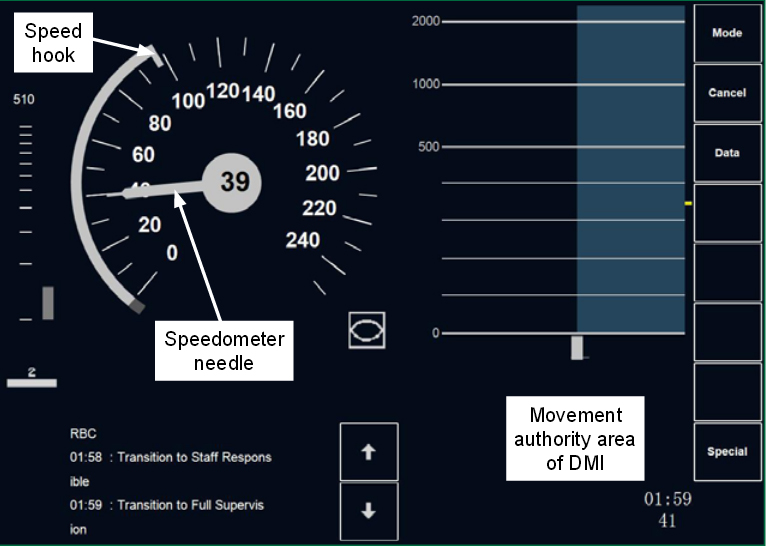
\includegraphics[scale=.25]{DMI.jpg}\\
Figure 4.1: \textit{Reference Driver Machine Interface \citep[p. 24]{RAIB12a}}
\end{center}

\subsubsection{ERTMS Systems Cab}
Given that ERTMS is a wholly digital solution, equipment which is used to maintain and supervise the system state is essential. Onboard a train, a cab containing ERTMS equipment provides the necessary infrastructure to operate a vehicle on an ERTMS-fitted line. This cab will typically contain the `European Vital Computer', a system which ``receives information from the track-side balise groups, interlocking [via GSM-R] and on-board odometry"\citep[p. 7]{NetworkRail15a}. In addition to the EVC, a `Juridical Recorder Unit', an on-board data recorder is installed which ``collects information about the performance of the train" \citep[p. 49]{RAIB12a}, plus a GSM-R Data Radio, which is a data modem maintaining a connection to the area base station, receiving data from the RBC.

On Class 158 units operating on the Cambrian Line, the ERTMS Systems Cab is publicly accessible, protected only with locks on the access door. This is a potential area of exposure where an attacker may be able to open the cab and attach equipment to the EVC or Juridical Recorder, interfering with the system without detection, especially if the train is relatively quiet. Another way, for example, would simply be to gain entry through social engineering, posing as a rail engineer.

Systems as critical as these should be placed, where possible, in locations where unauthorised access is minimal, for example in a driving cab. That said, a number of passenger trains other than the Bombarder Voyager and Alstom Pendolino family of trains, may be in the same position as the Class 158 if nationally deployed, due to space constraints. An overview of all the systems onboard a Class 158 and how it connects to ERTMS is detailed below.

\begin{center}
 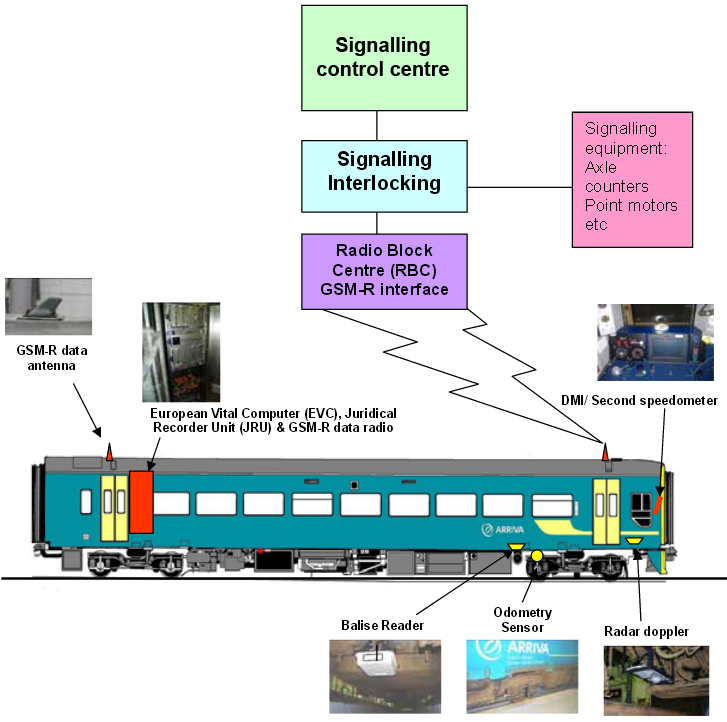
\includegraphics[scale=.3]{Cl158.jpg}\\
Figure 4.2: \textit{Modified hierarchy of systems on-board a train with communication links \citep[p. 51]{RAIB12a}}
\end{center}

\subsection{Case Study: Cambrian Line}
The UK has an active line operational under ERTMS, the Cambrian Line which runs from Shrewsbury, Shropshire to Aberystwyth, North Wales and Pwllheli. This line previously used a Radio Electronic Block Token (RETB) system due to the nature of the line. RETB is an outdated technology and due to ``radio frequencies that it operated on being withdrawn" \citep[p. 19]{RAIB12a}, it was selected in the ``early 2000's" as a candidate for ERTMS. The rollout was completed in March 2011, with the full line operating on ERTMS.

The Cambrian Line is fitted with ERTMS Level 2, with Class 158 Diesel Multiple Units operating on the track. The system was installed by Ansaldo STS, where the switchover from the former British Rail signalling system to ERTMS takes place near Shrewsbury.

\subsection{Vendor-specific Elements}
Successful ERTMS implementations have also been completed with one supplier responsible for the deployment, for example Siemens, Bombardier, Alstom or Ansaldo STS \citep{UNIFE15a}. Whilst ERTMS is a largely open standard, vendors may implement their own solutions to the specification. Trains may also be fitted with other vendor-supplied components, which will operate as specified under ERTMS systems interoperability, where the `back-end' makes an ERTMS implementation a Siemens or Alstom ERTMS deployment for example. The RBCs, interlocking and other constituent elements may use their own proprietary logic, to meet advertised capacity benefits and to maintain a commercial `edge'. These systems will communicate using open standards to the ERTMS `front-end' but again, from a security perspective, if there is a flaw in the implementation of the back-end, it may have unpredictable consequences as it could compromise the integrity of any security offered by systems which rely on the trust relationship.

There are no known open-source ERTMS implementations which are available for close scrutiny. However, the OpenETCS project is currently gaining interest in the open-source community for implementation, which is funded by the German Federal, French, Belgian and Spanish Governments. It is also commercially supported by SNCF, Lloyd's Register, Alstom and the UK ATOC members \citep{openETCS15a}.

As evidenced through recent vulnerabilities exposed in both commercial and open-source products for example, iOS and OpenSSL, open-source is sometimes not necessarily the solution, unless it has commercial backing and full dedication. Using an open-source approach would make the platform more transparent, reducing implementation costs and encourage collaboration.

Implementing this approach would open up this element of the Rail Systems market to greater competition and possibly promote joint efforts to improve security in the future development of ERTMS. This would, however, be conditional upon meeting the stringent quality assurance and accreditation processes specified by the international bodies.

Whilst there are some positive features with an open-source approach, it is considered unlikely to be further developed, given the investment in alternative proprietary systems, which have already been deployed.
\clearpage

\section{GSM-R}
The critical form of communications for ERTMS between train and trackside is performed through the Global System for Mobile Communication - Railway (GSM-R) specification, ratified by UIC as part of the EIRENE and MORANE projects. In the UK, Network Rail led a project to replace the ageing National Rail Network (NRN) and Cab Secure Radio (CSR) between 2009 and 2014, aiming to provide a communications system `functional across the whole of Britain'\citep{NetworkRail15c}.
\subsection{Overview}
GSM-R uses the well-established GSM Standard, but provides additional services to the standard GSM specification. The GSM-R frequency spectrum in the UK and Europe operates an uplink frequency of 876-880MHz and an downlink of 921-925MHz\citep[p. 36]{EIRENE-SRS}.

An end-to-end service is offered by GSM, whilst GSM-R provides specifications for network configuration and other features. GSM-R utilises the same cryptographic standard in its end-to-end connections as GSM, with the A5/1 cipher used for encryption of transmissions.
\subsection{Services Provided by GSM-R}
GSM provides services including:
\begin{itemize}[nolistsep]
\item Voice Broadcast and group call service
\item General Packet Radio Service (GPRS)
\item Data services at a range of available bandwidths
\end{itemize}
In addition to the services offered by GSM, GSM-R provides rail-specific applications including:
\begin{itemize}[nolistsep]
\item Emergency Calls
\item Multiple Driver communications
\item Rail-specific features, network parameters and standards
\item Exchanges of a number of location information packets between train and ground to support functional and location dependent addressing
\end{itemize}

Of potential use in GSM-R are pre-defined short messages which may be sent by driver and signaller, for example, `standing at signal'\citep{RSSB12a}, where the signaller may send a message to inform the driver to contact the signaller. GSM-R also supports group calls, should an emergency onboard a train take place, to inform drivers within the GSM-R area of the issue.

Whilst GSM-R offers a number of services, evidence suggests from investigative reports that, had it been introduced, GSM-R could have prevented a number of accidents, for example, Potter's Bar and Hatfield.

\subsection{Infrastructure}
Unlike the GSM topology where the mobile network is spread over an area, GSM-R is specifically fitted and concentrated to provide service line-side, with base stations located approximately every 3-4 kilometres along the track \citep[p. 509]{Dudoyer12a}. The topology of this network is designed such that at any point on the line, a train should be covered by two base stations. If one failed, it would still have GSM-R coverage provided by another base station \citep{GSM-R14a} \citep{Franekova11a}. These stations are connected to a fixed network which handles transmissions between entities.

Solutions such as repeaters and `leaky feeder' systems exist for use in tunnel environments to maintain the connection to the mobile network. Base stations, or masts, are connected to a fixed network which is responsible for routing, billing and other facilities. The fixed network also connects RBCs and controller equipment to the GSM-R network, which may include signaller communication equipment.

In addition, GSM-R has a single operator available per country, for example GSM-R GB for the UK network, and GSM-R DE for Germany. It is this feature which provides interoperability as the IDs of the Mobile Networks may be inserted onto the SIM Cards of the GSM-R radios to allow connections to these networks. It is this forward-thinking and application of an existing global standard which has allowed ERTMS to be rolled out internationally and enable interoperability.

\subsection{Contributions GSM-R has Made}
Taking the GSM standard and applying it to rail-specific applications inevitably improves safety. With coverage throughout the network in the UK, should an event occur which needs immediate attention, the driver is able to get the necessary help. Emergency calls, when initiated, drop all active calls that a signaller is participating in and initiates a group call, involving trains within the vicinity of the train making the emergency call. This makes them aware of the issue to allow appropriate action to be taken. Under the previous networks, there was no official way of supervising a train through voice and message communications, where a driver might have to change radio channels or perform some other actions to retain their connection. Today, a train is on a single network, and during its journey, moves into the new signaller's area of control seamlessly.

GSM-R has also opened the possibility for train to trackside communication, which is exactly what ERTMS leverages in order to mitigate the need for additional infrastructure and train equipment fitment costs.


\subsection{The Use of GSM-R as Part of ERTMS}
With the provision of a data service, GSM-R allows trains to send and receive data, a suitable means of communication for ERTMS, as a proven standard which has capabilities of maintaining a connection at high speed.
One additional benefit of using GSM-R for ERTMS applications is that, in the case of the UK, a national network exists for GSM-R, meaning that no additional line-side infrastructure is required other than that needed by ERTMS. This reduces the deployment cost significantly as there is no need to have two separate disjoint systems which ultimately serve the same purpose. All that would be required for an ERTMS deployment is the ERTMS track-side and onboard equipment.

The design of GSM-R also provides a robust platform for ERTMS to use, specifically that it has redundancy built in and supports vehicle speeds up to 500km/h. At present, GSM-R is the only communications standard that has been approved for rail applications. To introduce an alternative, based on the 3G and LTE standards may take considerable time, given that GSM had been in use for a number of years prior to the GSM-R Standard being ratified. Likewise, if GSM-R were to be phased out, the entire communication system may have to be replaced as LTE and 3G utilise IP, a protocol not used by GSM, with routing based on the GSM-R number allocated.

One concern, however, is that GSM-R is the `single point of failure' where if both cab radios failed, then the train would not be in a position to be supervised, and would not be able to run. Whilst ERTMS Level 2 has no requirement for line-side signals, this is an optional feature. The current platform does allow trains to move on a line where the GSM-R units on the vehicle have failed, albeit at a reduced speed.

\subsection{Weaknesses and Threats}
GSM-R as a derivative of the GSM standard relies not only on the same architectural principles, but also cryptographic properties. This, therefore, implies that any attack capable on the GSM standard could be applicable to GSM-R. A number of papers have been published, focussing on the A5/1 cipher in use within the GSM standard for encrypting traffic during transmission. GSM-R uses the same cipher for traffic, therefore traffic between train and base station may be intercepted and decrypted by an attacker. A paper presented at ACNS 2015 showed an optimised time-memory tradeoff attack breaking the A5/1 cipher within 9 seconds \citep{ACNS15a}. Moreover, Jain and Chaudhari demonstrate that with a pre-processing complexity of 2$^{48}$, the worst case would require between ``3-6 minutes", with approximately 280GB of diskspace, recorded over a 2 second window \citep{Arxiv13a}.

To mitigate this challenge, pre-computed rainbow tables reduce the search space for an attacker where Security Research Labs has made these available\footnote{Available at \url{https://opensource.srlabs.de/projects/a51-decrypt/files}}. Even in 2011, it was possible to reduce the complexity to $2^{38}$, with a memory complexity required of approximately 16GB, albeit with a 63\% success rate \citep{6062339}.

Under the premise, therefore, that GSM encryption is inherently weak by today's standards, it is possible to inject arbitrary data in the steam between train and trackside. With reference to mobile communications, this would simply break the principles of secrecy and privacy. When applied to rail applications, especially GSM-R data, however, an attacker would therefore be able to compromise the integrity of the train, with potentially catastrophic consequences, given that GSM-R is safety-critical and if violated in any way, could prove fatal.

Another possible attack is based on one presented by Paget at Defcon 2010, where an attacker was able to instead masquerade as a genuine mast and clients connected to this mast. Privacy and secrecy was undermined as the GSM standard allows clear transmissions, if the equipment is not capable of encryption \citep{Wired10a}. This specific attack in 2010 would have incurred a total equipment cost of approximately \$1,500 US Dollars -- something that would be significantly lower today given increased computational power at a lower cost.

It is not precisely clear if ERTMS requires a mobile network with ciphering enabled, or if it is simply a recommendation. If it is the former, then this attack would not be possible, but if it was the latter, then it might be possible to instead operate a mobile network acting as the Mobile Network ID `GSM-R GB' and see all train data in plaintext.

A more practical attack would be to jam one of the frequencies in use by the train on GSM-R, for example, the downlink frequency range, which would mean that if a RBC attempted to either issue an emergency stop, or shorten the Movement Authority for that unit, it would not be received, with possible fatal consequences. Here, a solution would be to use a heartbeat, where a train sends a heartbeat on a regular basis, which would be acknowledged by the base station and RBC. Upon receipt of this heartbeat, the train would consider both links stable. If a heartbeat response did not return in an acceptable time, then the train would attempt to resend it again, and if no further response is received, it would enter a `limp home' mode, restricting the movement of the train at the discretion of the driver. This solution would also apply if the attacker had blocked the uplink of the train, as the train would assume the downlink was also down. GSM-R on trains also includes a redundancy model where each train has two radios. If one fails, the other unit is used for communications. If both fail, and the train is not in a safe position to stop, it may proceed until a time it can reach coverage to contact the signaller, and report the fault when it is safe to do so. \citep{RSSB12a}. For ERTMS, the procedure isn't defined, so it may be possible that it relies on the timeout (if one is set for ERTMS) and then handle it appropriately.

On balance, whilst the attack by Paget is a `quick win', using the rail infrastructure and being a passive attacker has a greater payoff, as less physical equipment would be required, which would otherwise arouse suspicion. Even if this were possible, it might have limited success due to the number of external factors to consider, for example, the resilience of GSM-R and breaking A5/1. DB Netze states that ``if disruptions or outages ... occur in the GSM-R Network,... [drivers] can use public roaming with the P-GSM D network" \citep{DBNetze12a}. DB currently has 1,437km \citep{UNIFE15a} of track under ERTMS, with some deployments being L2 enabled. If the same principle for the cab radio applies to the GSM-R radio used for ERTMS traffic, then there is another exposure of a critical system to `the world'. Such an attack in a similar fashion to the Jeep uConnect scenario could be applied, if the train security was based on the GSM-R network. \citep{uconnect15a}.

\subsection{Looking to the Future of GSM-R}
GSM itself as a technology and standard supports only a small bandwidth compared to modern alternatives \citep{RailEngineer13b} and is over 20 years old. Mobile communications now leverage standards such as 3G and LTE which support higher bandwidths. However, as seen with Wi-Fi, the higher the bandwidth made available, the smaller the transmission range. In a city or clustered region, coverage will be strong. However, when looking at rail, where lines may go through particularly rural areas, additional infrastructure to support rail applications and use would be required, which would incur significant cost.

Research has been undertaken in assessing the relative feasibility of using LTE in rail applications, where the use of 3G and LTE would improve quality of communications, whilst reducing the cost, given technological advancements in these areas. As part of the renewal of rail communication infrastructure to cope with future needs, it would be likely that LTE and 3G technologies are used to ensure ERTMS remains future-proof and dynamic in a world that is technologically advancing in rail applications.

Such communication standards could also provide a means of monitoring a train's condition remotely and perform a real-time diagnosis of a train's operational systems. This is not currently possible without vendors installing their own systems, which use Wi-Fi and 3G en-route to send such data to the vendors to identify maintenance needs. In 2013, Network Rail admitted that GSM-R is a limiting factor in the deployment of ERTMS for Thameslink and Crossrail, with current capacity offered by GSM-R restricted to handling ``60 trains simultaneously" \citep{FT13a}. However, for future use, GSM-R may not be a suitable platform, which limits further possible growth, restricting potential developments of ERTMS, for example, restricting capacity and speed due to constraints imposed by GSM-R.

\subsection{Research in the Future of GSM-R}
Research has already begun to assess the feasibility and challenges to deploying next-generation communications for rail-use. Kim et al evaluated the challenges presented as a train would be handed over from one RBC to another with LTE \citep{Kim14a}. They observe that the use of LTE would bring a number of benefits to the railway with additional bandwidth and meet the passenger needs of the future. One of the particular challenges they note is that RBC-RBC handover for a train is a `hard' process, where the connection is terminated and re-established with the accepting RBC, with handovers potentially at risk of not succeeding first time. The approach by the researchers is to use a soft-handover process, where the train will connect to two base stations and perform the handover. Under ERTMS, however, this is not required as a train will only perform the handover, if and only if the accepting RBC is prepared to accept the train. If the train has multiple radios, then it will attempt to retain a connection with one RBC whilst connecting to the accepting RBC to carry out the handover process.

Calle-Sanchez et al look at the challenges of implementing LTE for the railway as a whole \citep{CalleSanchez12a}. One of the key challenges for LTE-R would be adding functionality that LTE currently does not support, in a similar way that GSM-R required additional functionality not provided by GSM. LTE, however, uses a very different architecture, being IP-based, compared to GSM-R. This, however, will again take a number of years to establish both base-line architectures and specifications on which to build the ``natural evolution to GSM-R".

\clearpage

\section{EuroRadio}
GSM-R is the base layer of the ERTMS stack, which is used to communicate between train and track-side. To process data arriving and present it in a format accessible to the application, an additional layer is required. Within the ERTMS `stack', below, the EuroRadio layer is situated immediately between the (open) communications layer, GSM-R, and the Application Layer.

This section examines the protocol used within the EuroRadio connection process, the cryptographic properties it holds, and a formal analysis of both.
\begin{center}
 \includegraphics[scale=.5]{ERTMSStack.eps}\\
Figure 6.1: \textit{Train-side ERTMS `Stack' with appropriate fields used}
\end{center}

\subsection{The EuroRadio Protocol}
The EuroRadio protocol is designed to be a means to secure communications between ERTMS entities over an otherwise open communications link (GSM-R). EuroRadio provides a way to authenticate and verify the integrity of data between these entities, to prevent forgery of messages in addition to forming a trust relationship to ensure messages conversed are genuine. The EuroRadio protocol is used to meet a number of requirements in order to be compliant with EN50159 (Safety-related communications in transmission systems), utilised in both train $\leftrightarrow$ trackside and RBC $\leftrightarrow$ RBC communications.

The EuroRadio layer sits immediately between the open communication (GSM-R) and Application Layer, where data received is verified and passed to the Application Layer. As part of the header, a definition of what the data held within this `packet' is specified, whether it is an authentication message or data\footnote{This message is sent following a successful Identification and Authentication challenge and the EuroRadio connection is established.}. When data is being sent by an ERTMS entity, it generates a cryptographic  Message Authentication Code (MAC) which is then part of the EuroRadio data `frame' which is passed to the GSM-R layer for transmission. Upon receipt by the receiving entity, the MAC is verified to ensure that it has arrived in a correct state. This MAC can only be generated and verified when both parties have a shared key.

The shared key is exchanged using an Identification and Authentication (I\&A) handshake protocol, whereby a successful exchange results in a symmetric key being derived successfully by both parties. After this exchange, a EuroRadio connection is established, and higher layers may use this connection and layer to exchange authenticated messages.
\subsection{EuroRadio Handshake Connection Protocol}
To establish the secure connection between ERTMS entities, the train would initiate the EuroRadio connection protocol, sending a 64 bit nonce with some standard data. The RBC to which it connects generates its own 64 bit nonce, derives the session key using the stored train key based on the train nonce and its nonce, ensuring key freshness. This nonce is sent to the train, accompanied by a MAC to demonstrate the requisite proof of work that it has knowledge of the key.

The train verifies this MAC by deriving the session key itself using the same process as the RBC. If the MAC is correct, then the protocol proceeds with the next step, which involves sending a third data packet to confirm that the train itself has knowledge of the key. When the RBC verifies this, and it is proven correct, an `Authentication Response' message is sent and the connection is established.

What is pivotal to the protocol is that the train has its own key which can be considered as a `seeding key', used to derive future session keys. Whilst this is private to the train, it is held by a Key Management Centre, which is nationally operated. If a RBC is expected to ever be responsible for a train, the key is then shared and distributed so that the RBCs may generate the session key themselves. Key Management is further explored in Section 8.1.\\
The full handshake protocol is listed below.

\begin{algorithm}[H]
\floatname{algorithm}{EuroRadio Protocol}
\renewcommand{\thealgorithm}{}
\caption{Steps that an ERTMS Entity would undertake to establish a connection}
T: Train, R: Radio Block Centre, $K_{MAC}$: Train Key, $KS_{MAC}$: Session Key
\label{EuroRadio Protocol}
\begin{algorithmic}[1]
\STATE $T\rightarrow{R}$ : \{\texttt{ETY},\texttt{MTI}$\gets$AU1, \texttt{DF}$\gets$0, Sender ETCS ID, Safety Feature, R$_T$\}.
\STATE $R\rightarrow{T}$ : \{\texttt{ETY},\texttt{MTI}$\gets$AU2, \texttt{DF}$\gets$1, Responding ETCS ID, Accepted Safety Feature, R$_{RBC}$,\\CBC-MAC($KS_{MAC}$, (Length, Destination Address, \texttt{ETY}, \texttt{MTI}, \texttt{DF}, Responding ETCS ID, SaF, R$_{RBC}$, R$_T$, Destination Address, Padding))\}
\STATE $T\rightarrow{R}$ : \{`\texttt{000}', \texttt{MTI}$\gets$AU3, \texttt{DF}$\gets$0,\\CBC-MAC($KS_{MAC}$, (Length, Destination Address, `\texttt{000}', \texttt{MTI}, \texttt{DF}, $R_T$, $R_{RBC}$, Padding))\}
\STATE $R\rightarrow{T}$ : \{`\texttt{000}', \texttt{MTI}$\gets$AR, \texttt{DF}$\gets$1,\\CBC-MAC($KS_{MAC}$,(Length, Destination Address, `\texttt{000}', \texttt{MTI}, \texttt{DF}, Padding))\}
\end{algorithmic}
$\Rightarrow$ \textit{Connection Established}
\end{algorithm}
\begin{center}
\vspace{-0.5cm}
Figure 6.2: \textit{EuroRadio Protocol for Connection Establishment}
\end{center}

As part of the handshake protocols, set values, for example, the ETCS ID type and Message Type are statically set, with the values for the non-dynamic variables shown below:

\begin{itemize}[nolistsep]
\item The ETCS ID Type (\texttt{ETY}) may be one of the following values:\\
Bit \tab\tab\tab\space: Reference Value\\
\texttt{000. ....} : Radio Infill Unit\\
\texttt{001. ....} : RBC\\
\texttt{010. ....} : Engine\\
\texttt{011. ....} : Reserved (Balise)\\
\texttt{100. ....} : Reserved (Field element e.g. Level Crossing)\\
\texttt{101. ....} : Key Management entity\\
\texttt{110. ....} : Interlocking-related entity
\item The Message Type ID (\texttt{MTI}) may be one of the following values:\\
\texttt{AU1} : First Authentication SaPDU\\
\texttt{AU2} : Second Authentication SaPDU\\
\texttt{AU3} : Third Authentication SaPDU\\
\texttt{AR} : Authentication Response\\
\texttt{DT} : Data Payload
\item The Direction Flag (\texttt{DF}) may be one of two values:\\
\texttt{0} : Session Initiator\\
\texttt{1} : Session Responder
\item The Safety Feature, according to the EuroRadio FIS is specified as `Single DES with modified MAC Algorithm 3', with other values reserved. In contrast, Italian Specifications include a value for CRC authentication \citep{Ferrovia09a}.
\item R$_T$ and R$_{RBC}$ are 64-bit nonces, generated locally.
\end{itemize}

\subsection{MAC Algorithm Protecting Messages}
The MAC algorithm in use by EuroRadio is not one derived by the ratification committee; rather a modified version of `MAC Algorithm 3', which is defined within ISO9797 \citep{ISO9797-1}. This standard outlines a number of keyed MAC algorithms, where Algorithm 3 is a block chained MAC algorithm. This algorithm uses a single DES key for the $n-1$ blocks of the plain text, and performing in the last block a DES encryption transformation using two distinct keys, prior to outputting this block as the MAC.\\
The version used by EuroRadio, however, uses three distinct keys in an Encrypt-Decrypt-Encrypt process for the final block transformation.

One may consider that this a step forward as the MAC algorithm used also has additional features differentiating it from the standard MAC Algorithm. Matthew Green \citep{Green13a} has previously written on how CBC-MAC algorithms can be improved. One inclusion was to prepend the data held within the MAC with the length, also known as `length-prepend MAC'. An attacker would not then be able to intercept the message, by, say, adding zeros to the start. This reduces the space for an attacker to exploit - and when added to a destination address embedded into the MAC, the result is that an attacker may not relay messages, as the destination address will mismatch.

These additional measures mean that if, by chance, a collision exists from the same nonces being exchanged, the message cannot be replayed as the destination address within the MAC is incorrect, as well as the direction flag. The MAC generation process is explored further in the figure below:

\begin{algorithm}[H]
\floatname{algorithm}{CBC-MAC Calculation used in EuroRadio}
\renewcommand{\thealgorithm}{}
\caption{Algorithm to calculate a CBC-MAC for a given message}
M: Message to CBC-MAC, where $M_1,M_2,...,M_q \in M$ are 64-bit blocks\\
\textit{Let} $K$ = $(K_1,K_2,K_3)$, each a 64-bit DES Key.\\
\textit{Let} $\bigoplus$ denote the XOR operation.

\label{MAC Algorithm}
\begin{algorithmic}[1]
\STATE Let $H_0$ be 64-bits of zeros.
\FOR {($i=1, i < q$)}
	\STATE $H_i$ = E$_{K1}$($H_{i-1} \bigoplus X_i$)
\ENDFOR
\STATE $H_q$ =  E$_{K3}$(E$^{-1}_{K2}$,(E$_{K1}$,($H_{q-1} \bigoplus X_q$)))
\STATE CBC-MAC(M) = $H_q$
\end{algorithmic}
$\Rightarrow$ \textit{MAC Output for sending with messgae}
\end{algorithm}
\begin{center}
\vspace{-0.5cm}
Figure 6.3: \textit{MAC Calculation of a given message M}
\end{center}

\subsubsection{Importance of Proof of Knowledge}
In the second step of the protocol, an attacker may be in a position to react faster than a RBC, and assuming the GSM-R connection has been intercepted and actively allowing interaction by the attacker, they may be able to reply to the message and send a message, possibly a previous capture of a handshake by the train which uses the same train nonce. This passes the MAC verification, given the nonce sent by the train is the same as that represented within the MAC. What this attack would do is cause the train to incorrectly derive the session key with the wrong nonce being given by the attacker. The third authentication step would therefore fail. This is due to the RBC attempting to verify the MAC with what is a fresh and new session key, but the train has created a MAC with an invalid session key, causing a mismatch upon MAC validation.
The connection would then be rejected by the RBC, and the train would need to attempt another EuroRadio connection handshake before continuing.
Likewise, the third authentication step is critical, as an attacker may replay another session, and where the MAC mismatches, shows the entity either incorrectly derived the key, or did not know the original key in the first place and was attempting to see if a MAC would have been accepted by the receiving party.

It is this proof of knowledge that allows the train and the RBC to have trust in each other, and that the key they hold is a good key for that particular session.


\subsubsection{Threats to EuroRadio as a Protocol}
Under EN50159, adequate protection against the following threats must be provided \citep{EN50159}:
\begin{itemize}[nolistsep]
\item Repetition, where a message is sent more than once
\item Deletion, where a message sent is not received by the other party
\item Insertion, where a new message is injected into a message stream
\item Resequencing, where messages may arrive out of order
\item Corruption, where the contents of the message may have been modified inflight
\item Delay, where the message is received at a time later than expected
\item Masquerade, where a forged message is accepted as being authentic with the attacker impersonating a valid entity participating in the connection
\end{itemize}

EuroRadio, as it stands in the specification, only fulfils a few of the requirements set down by the EN50159 standard, relying on the upper Application Layer level to provide the appropriate protection for which it is not designed. These assumptions and levels of protection offered by the Application Layer will be discussed fully in Section 7.2.1. Outside of the specification, the keys are fresh as they are generated at time of connection, meaning that the lifetime of the keys is relatively short, given that, at the time of the handover between the two RBCs, the active connection is torn down \citep[Section 3.15.1.3]{SUBSET-026-3} and a new connection is set up specific to the accepting RBC.

For EuroRadio, the threat/defence matrix for EN50159 compliance was compiled:

\begin{center}
\vspace{-1.0cm}
Table 6.4: \textit{Threat/Defence Matrix for EuroRadio, marked against EN50159}
\end{center}

It is also important to note that within the EuroRadio specification, the Safety Feature (SaF) does not need to be set to `CBC-MAC with Modified MAC Algorithm 3'. Italian Specifications for ERTMS specify the use of Cyclic Redundancy Check (CRC) which is easier to attack, given it is a linear function, which requires little effort to break. For a CRC, given a CRC-MAC of message $m$, an attacker may XOR their own bits into the CRC, which could result in allowing a train's Movement Authority to exceed its limit, and potentially lead to a collision \citep{Ferrovia09a} \citep{Lockstone00a}.

\subsection{Tools Used in Formal Analysis}
In order to model the EuroRadio connection protocol, the Proverif\footnote{\url{http://prosecco.gforge.inria.fr/personal/bblanche/proverif/}} protocol verifier was used. This tool is an ``automatic cryptographic protocol verifier,..., based on the representation of the protocol by Horn clauses" \citep{Proverif}.

Given a model of a protocol, Proverif will automatically perform `runs' of the protocol, and identify whether there are exposures to possible attacks, including replay or forgery attacks. With this knowledge, if an attack can be found, Proverif will provide a proof through logical statements. Otherwise, it will identify whether a given property holds, or if it cannot be proven. These attacks are given in the form of queries, which relate to events within the model, such that if one event is reached, it can identify whether there was a corresponding event, assessing the (non)injective property for validity.

The results that Proverif provide are in the context of the protocol itself and as an implementation of the model, not of the cryptography used within the protocol. This, therefore, means that should a protocol be proven to be secure by Proverif, it may have some other vulnerabilities outside of the scope of the verifier, such as weak encryption, or poor key derivation. The use of Cryptography within GSM-R and ERTMS is discussed in more detail in Sections 5.6 and 6.8.
\subsection{Formally Modelling the EuroRadio Protocol}
Using the Proverif tool, it is possible to translate the EuroRadio protocol into a program which the verifier can run. For this, the GSM-R `wrapper' is not considered - it is assumed that a train has an active GSM-R connection to a base station, and that there is no active EuroRadio connection between train and trackside. Thus, a free open channel is defined, with additional definitions provided for operations which encrypt, decrypt and create a MAC of a given message with a key respectively. These are simply skeleton functions with no functionality defined in terms of cryptographic algorithms. The MAC algorithm was implemented in Proverif as a two parameter function which takes a key and a message and performs some transformation to create a deterministic result. As mentioned above, Proverif doesn't concern itself with the implementation of functions in this way, it is a way of stating that these functions exist, and to form tuples representing this relationship or function use.

The protocol also uses a number of predefined variable values, such as the message type, and direction flags, which are defined as `DATA' constructs. These are zero parameter functions which produce some output which represents that construct. The Proverif model created also includes a `private' secret, to assess whether messages encrypted by the derived key are able to be intercepted by the attacker, and the raw value obtained.

Proverif also allows local binding to the entity, including, in the case of the EuroRadio model, the generation of the session key, such that an attacker cannot explicitly see a value. During implementation of this model, sanity checks were added to ensure that a full run-through was possible, by adding queries to identify if an attacker was able to see an event firing, which signified the end of the protocol and connection establishment succeeding.

Data transferred between entities are represented with \texttt{in} or \texttt{out} clauses, which indicate dataflow. These use a fixed channel, \texttt{c}, which is defined as a free open channel, and removes any ambiguity of protection offered by the lowermost GSM-R communications layer. This model therefore focusses purely on the EuroRadio protocol and nothing else.

MAC validation also required skills in the application of how OCaml uses handles tuples to generate a MAC and compare and match those to verify a genuine MAC. Once this was completed, the protocol modelled in Proverif was validated against the EuroRadio specification to ensure that it was accurate and implemented the protocol correctly. As Proverif does not have a notion of bits in this model, the padding added as part of the MAC to make it into an appropriate multiple of the key length, was omitted.

One additional, useful, feature of the Proverif verifier is that in specific stages of a protocol, such as once the handshake is completed, events may be `fired', and in a protocol involving two parties, it is possible to query whether one event is `fired' as the result of another. The model would query whether an attacker had been able to obtain the raw value of the secret sent, in addition to establishing whether the trust relationships exist. In this model, a number of different events are used, including \texttt{event} which has a name and value, which requires no injective property for a relationship. Injective relationships may be represented using the \texttt{evinj}\footnote{The Proverif model for the entities continues to use \texttt{event} where queries use \texttt{evinj}.} query to test the inferred relationship properties to verify if they hold. Other queries used the \texttt{attacker} query construct to identify whether an attacker eavesdropping on the channel was able to achieve a state where they were able to obtain the secret values passed down the channel. This would prove whether or not secret data was passed in the clear.

\subsubsection{Processes in Proverif}
In order to `run' the Proverif model, a process model must be created. In the case of EuroRadio, this would be an infinite number of trains, with an infinite number of ETCS IDs, and similarly for the RBCs to identify whether there is a possibility of messages being replayed in different circumstances. This allows the model to simulate an attacker listening to an arbitrarily high number of communications, for example at termini, to identify if it is possible to replay messages at some point in time, or establish the key.

\begin{verbatim}
process
	( !new train_etcs_id;!Train | !new rbc_etcs_id;!RBC )
\end{verbatim}

\subsection{Results}
To ensure that the EuroRadio connection protocol is analysed thoroughly using formal means, several questions were formulated, and translated into corresponding Proverif queries. These queries included:
\begin{itemize}[nolistsep]
\item Is it possible for the attacker to obtain the secret value?
\item If a train has trust in the key, does the RBC have trust in it?
\item If a RBC has generated a key, does the train trust that key?
\item Is there a direct relationship between a RBC accepting a message and a train having sent it?
\item Does the protocol allow replay attacks?
\end{itemize}

With these queries modelled in Proverif, the following results were generated:
\subsubsection{Secrecy of Secret Value}
\begin{verbatim}
-- Query not attacker:secret[]
Completing...
Starting query not attacker:secret[]
RESULT not attacker:secret[] is true.
\end{verbatim}
The result provided by Proverif means that, despite a number of protocol runs, the attacker would be unable to establish the value of the secret, which is beneficial, as it shows that the secret is never communicated in plain text, with its ciphertext pair. This shows that in principle, the encryption used is sufficiently strong to prevent simple eavesdropping on the link.

\subsubsection{RBC Trust in the Train}
\begin{lstlisting}
-- Query evinj:rbcTrustTrain(x_6420) ==> evinj:trainKeyTrust(x_6420)
Completing...
Starting query evinj:rbcTrustTrain(x_6420) ==> evinj:trainKeyTrust(x_6420)
goal reachable: begin:trainKeyTrust(genSessionKey(trainNonce_17[!2 = @sid_8165,!1 = @sid_8166],rbcNonce_27[!3 = endsid_8167,!2 = @sid_8168,!1 = @sid_8169],getKey(train_etcs_id_16[!1 = @sid_8166]))), recv_MAC_20 = mac(genSessionKey(trainNonce_17[!2 = @sid_8165,!1 = @sid_8166],rbcNonce_27[!3 = endsid_8167,!2 = @sid_8168,!1 = @sid_8169],getKey(train_etcs_id_16[!1 = @sid_8166])),((PAYLOAD_LENGTH(),train_etcs_id_16[!1 = @sid_8166],RBC_ETCS_ID_TYPE(),AU2(),DF_RESP(),rbc_etcs_id_26[!2 = @sid_8168,!1 = @sid_8169],SAF()),rbcNonce_27[!3 = endsid_8167,!2 = @sid_8168,!1 = @sid_8169],trainNonce_17[!2 = @sid_8165,!1 = @sid_8166],train_etcs_id_16[!1 = @sid_8166])), rbcN_19 = rbcNonce_27[!3 = endsid_8167,!2 = @sid_8168,!1 = @sid_8169], recv_rbc_etcs_id_18 = rbc_etcs_id_26[!2 = @sid_8168,!1 = @sid_8169], @sid_430 = @sid_8165, @sid_429 = @sid_8166, @occ10_6852 = @occ_cst() -> end:endsid_8167,rbcTrustTrain(genSessionKey(trainNonce_17[!2 = @sid_8165,!1 = @sid_8166],rbcNonce_27[!3 = endsid_8167,!2 = @sid_8168,!1 = @sid_8169],getKey(train_etcs_id_16[!1 = @sid_8166])))
RESULT evinj:rbcTrustTrain(x_6420) ==> evinj:trainKeyTrust(x_6420) is true.
\end{lstlisting}
Here, Proverif performs a run of the protocol as a genuine entity, and is able to reach the state where the train has completed the adequate proof of work to demonstrate that it has knowledge of the key. Given that the train is the only non-RBC entity that could have this key, it can therefore be trusted.

This injective relationship shows that, for this particular session, the RBC must have trust in the train with the key it has derived.\\

\subsubsection{Train Trust in the RBC Generated Key}
\begin{lstlisting}
-- Query evinj:trainKeyTrust(x_4440) ==> evinj:rbcGenSessionKey(x_4440)
Completing...
Starting query evinj:trainKeyTrust(x_4440) ==> evinj:rbcGenSessionKey(x_4440)
goal reachable: begin:rbcGenSessionKey(genSessionKey(trainNonce_17[!2 = endsid_6400,!1 = @sid_6401],rbcNonce_27[!3 = @sid_6403,!2 = @sid_6404,!1 = @sid_6405],getKey(train_etcs_id_16[!1 = @sid_6401]))), trainN_30 = trainNonce_17[!2 = endsid_6400,!1 = @sid_6401], recv_train_etcs_id_29 = train_etcs_id_16[!1 = @sid_6401], sent_ETCS_ID_TYPE_28 = sent_ETCS_ID_TYPE_6402, @sid_829 = @sid_6403, @sid_828 = @sid_6404, @sid_429 = @sid_6405, @occ22_5191 = @occ_cst() & attacker:sent_ETCS_ID_TYPE_6402 -> end:endsid_6400,trainKeyTrust(genSessionKey(trainNonce_17[!2 = endsid_6400,!1 = @sid_6401],rbcNonce_27[!3 = @sid_6403,!2 = @sid_6404,!1 = @sid_6405],getKey(train_etcs_id_16[!1 = @sid_6401])))
RESULT evinj:trainKeyTrust(x_4440) ==> evinj:rbcGenSessionKey(x_4440) is true.
\end{lstlisting}
The result established here shows that, given the RBC has generated a session key, the train is now able to establish trust in the key. This confirms that the RBC has completed some proof of work to demonstrate that it has knowledge of the shared key.

It is important to note that the RBC is the first entity to generate the key and, if an attacker were to intercept and modify the nonce sent by the RBC, it would affect the key derivation, which would lead to this property not holding.\\

\subsubsection{RBC Accepting Data from a Train}
\begin{lstlisting}
-- Query evinj:rbcAcceptsData(x_2643) ==> evinj:trainSendData(x_2643)
Completing...
Starting query evinj:rbcAcceptsData(x_2643) ==> evinj:trainSendData(x_2643)
goal reachable: begin:trainSendData((DT(),trainData_22[recv_MAC_20 = mac(genSessionKey(trainNonce_17[!2 = @sid_4423,!1 = @sid_4424],rbcNonce_27[!3 = endsid_4425,!2 = @sid_4426,!1 = @sid_4427],getKey(train_etcs_id_16[!1 = @sid_4424])),((PAYLOAD_LENGTH(),train_etcs_id_16[!1 = @sid_4424],RBC_ETCS_ID_TYPE(),AU2(),DF_RESP(),rbc_etcs_id_26[!2 = @sid_4426,!1 = @sid_4427],SAF()),rbcNonce_27[!3 = endsid_4425,!2 = @sid_4426,!1 = @sid_4427],trainNonce_17[!2 = @sid_4423,!1 = @sid_4424],train_etcs_id_16[!1 = @sid_4424])),rbcN_19 = rbcNonce_27[!3 = endsid_4425,!2 = @sid_4426,!1 = @sid_4427],recv_rbc_etcs_id_18 = rbc_etcs_id_26[!2 = @sid_4426,!1 = @sid_4427],!2 = @sid_4423,!1 = @sid_4424])), recv_MAC_20 = mac(genSessionKey(trainNonce_17[!2 = @sid_4423,!1 = @sid_4424],rbcNonce_27[!3 = endsid_4425,!2 = @sid_4426,!1 = @sid_4427],getKey(train_etcs_id_16[!1 = @sid_4424])),((PAYLOAD_LENGTH(),train_etcs_id_16[!1 = @sid_4424],RBC_ETCS_ID_TYPE(),AU2(),DF_RESP(),rbc_etcs_id_26[!2 = @sid_4426,!1 = @sid_4427],SAF()),rbcNonce_27[!3 = endsid_4425,!2 = @sid_4426,!1 = @sid_4427],trainNonce_17[!2 = @sid_4423,!1 = @sid_4424],train_etcs_id_16[!1 = @sid_4424])), rbcN_19 = rbcNonce_27[!3 = endsid_4425,!2 = @sid_4426,!1 = @sid_4427], recv_rbc_etcs_id_18 = rbc_etcs_id_26[!2 = @sid_4426,!1 = @sid_4427], @sid_430 = @sid_4423, @sid_429 = @sid_4424, @occ14_3186 = @occ_cst() -> end:endsid_4425,rbcAcceptsData((DT(),trainData_22[recv_MAC_20 = mac(genSessionKey(trainNonce_17[!2 = @sid_4423,!1 = @sid_4424],rbcNonce_27[!3 = endsid_4425,!2 = @sid_4426,!1 = @sid_4427],getKey(train_etcs_id_16[!1 = @sid_4424])),((PAYLOAD_LENGTH(),train_etcs_id_16[!1 = @sid_4424],RBC_ETCS_ID_TYPE(),AU2(),DF_RESP(),rbc_etcs_id_26[!2 = @sid_4426,!1 = @sid_4427],SAF()),rbcNonce_27[!3 = endsid_4425,!2 = @sid_4426,!1 = @sid_4427],trainNonce_17[!2 = @sid_4423,!1 = @sid_4424],train_etcs_id_16[!1 = @sid_4424])),rbcN_19 = rbcNonce_27[!3 = endsid_4425,!2 = @sid_4426,!1 = @sid_4427],recv_rbc_etcs_id_18 = rbc_etcs_id_26[!2 = @sid_4426,!1 = @sid_4427],!2 = @sid_4423,!1 = @sid_4424]))
RESULT evinj:rbcAcceptsData(x_2643) ==> evinj:trainSendData(x_2643) is true.
\end{lstlisting}
A full run of the protocol as a genuine entity was then required to enable this property to be reached. An attacker cannot reach this state by constructing a message - there is an injective relationship between the train having sent some data and a train receiving it.\\

\subsubsection{RBC Accepting Replayed Messages}
\begin{lstlisting}
-- Query not ev:rbcAcceptsData(x_45)
Completing...
Starting query not ev:rbcAcceptsData(x_45)
goal reachable: end:rbcAcceptsData((DT(),trainData_22[recv_MAC_20 = mac(genSessionKey(trainNonce_17[!2 = @sid_1988,!1 = @sid_1989],rbcNonce_27[!3 = @sid_1990,!2 = @sid_1991,!1 = @sid_1992],getKey(train_etcs_id_16[!1 = @sid_1989])),((PAYLOAD_LENGTH(),train_etcs_id_16[!1 = @sid_1989],RBC_ETCS_ID_TYPE(),AU2(),DF_RESP(),rbc_etcs_id_26[!2 = @sid_1991,!1 = @sid_1992],SAF()),rbcNonce_27[!3 = @sid_1990,!2 = @sid_1991,!1 = @sid_1992],trainNonce_17[!2 = @sid_1988,!1 = @sid_1989],train_etcs_id_16[!1 = @sid_1989])),rbcN_19 = rbcNonce_27[!3 = @sid_1990,!2 = @sid_1991,!1 = @sid_1992],recv_rbc_etcs_id_18 = rbc_etcs_id_26[!2 = @sid_1991,!1 = @sid_1992],!2 = @sid_1988,!1 = @sid_1989]))

... trace output ...

The event rbcAcceptsData((DT(),trainData_22_2500)) is executed.
A trace has been found.
RESULT not ev:rbcAcceptsData(x_45) is false.
\end{lstlisting}
Here, it is evident that the RBC will accept any data message it is receiving as a replay, where the Proverif code was designed such that it was required to perform two inputs of the same data before reaching this event. Thus, the EuroRadio protocol is, most critically, not immune to replay attacks by an attacker listening to communications.

An adequate defence against this could be implemented in the form of either a time-stamp or a sequence number, so that replayed messages could be identified and rejected appropriately if there is any doubt of replay or out of sequence packets. If the sequence number was, for example, four bytes in length, this would provide a sufficiently large number which would be difficult for the attacker to guess and replay messages upon wraparound.  Time-stamps have the added benefit that they restrict the validity of a message. If there was a case where the sequence number would wraparound, the accompanying time-stamp would be invalid -- if an attacker tried to make the time-stamp valid, it would require a corresponding valid MAC. Time-stamps also provide a level of defence against delayed messages. If messages were intercepted and forwarded after a substantial delay for an extended amount of time, the effectiveness of this defence is reduced. A heartbeat could therefore be used, which establishes delay thresholds, given as a train approaches a mast, which one would expect would minimise delays in communication. When coupled with train location data, it is possible to understand the precise location of a train and if the delay encountered for a message response is acceptable.

One other consideration is that the EuroRadio handshake protocol is best represented as a state machine, where the messages must follow set transitions to proceed - if any of the authentication steps were to be replayed, this would cause an out-of-state error, which the protocol deems as replay. Once the connection is established, however, it is up to the Application Layer to detect replay, not EuroRadio.

Moreover, outside of the Proverif model, deletion of messages is also, perhaps, possible by an attacker, for example, by jamming the GSM-R connection. Messages like acknowledgements or Movement Authorities will therefore fail to be received by the appropriate party. Within the specification, there is some tolerance. This, however, is not perfect, as it again relies on the Application Layer to detect it. Again, the defences proposed in this paper resolve the threat of replay attacks, if implemented at the EuroRadio level, and would prevent deletion attacks, as any attempt of deleting messages would show a visible gap between sequence numbers of messages.

Given that the specifications for the EVC are unavailable from the manufacturers, it is a likely assumption that the EVC will use modern hardware, with commonplace processors, such as Intel/AMD server-grade CPUs for reliability and performance. If an attacker was able to replay one message, they would be able to replay a thousand. If these messages are received by the train in a very short space of time, the EuroRadio layer will queue these whilst they are being verified before passing valid messages to the Application Layer. At any time, an order to shorten the Movement Authority of a train may be genuinely sent, but if the queues are not of sufficient size and are being flooded, it may be ignored. If the Application Layer is blocked parsing the messages, it may be possible to cause the train application processes to be in a state of resource contention where it they are not able to progress due to the allocation of resources verifying the MACs and processing the information given to it. This could lead to a state where safe operation of the train is at risk.
\clearpage

\subsection{High-Priority Messages}
The EuroRadio Specification includes the requirement for sending emergency messages, called `high-priority' messages. These use a different SaPDU compared to the Data SaPDUs, the High Priority (HP) SaPDU.
\subsubsection{Overview}
High-priority messages are limited in their scope to only allow a strict subset of the ERTMS message specifications to be sent as a high-priority message. These messages are discussed in the next section.\\
The justification behind high-priority messages between the RBC and OBU is ``to get a quick reaction" \citep[Section 3.10.1.1.1]{SUBSET-026-3}. To facilitate this `quick reaction' by the train, DMI and driver, high-priority messages use a different path to reach the ATP Application Layer from the\\EuroRadio layer, which bypasses any message queues and MAC validation, to ensure it is received. The specifications state that high-priority messages do not require a corresponding MAC \citep[Section 7.1.7]{SUBSET-037}, and it is up to the Application Layer to verify the message type is a valid message. It is worth noting, however, that high-priority messages may be sent with normal priority, accompanied by a MAC, and all acknowledgements are also then sent as normal priority messages, which would be appropriately MAC'd. The threat here is if a train is slow to process messages, and has a number of messages in its queue, it may take time for an emergency stop message to be processed, which could lead to a potential crash. This bypass of message queues for high-priority messages is therefore justified, as an emergency message might sit in a queue for an unnecessary period of time, but more importantly, what about bypassing the verification of message MACs?

The diagram below demonstrates how normal priority messages are queued during send and receive operations, however, the queues are bypassed for high-priority messages. Although the diagram shows that high-priority messages bypass the EuroRadio layer, they only bypass the MAC validity checks in the EuroRadio layer (highlighted with an *).

\begin{center}
 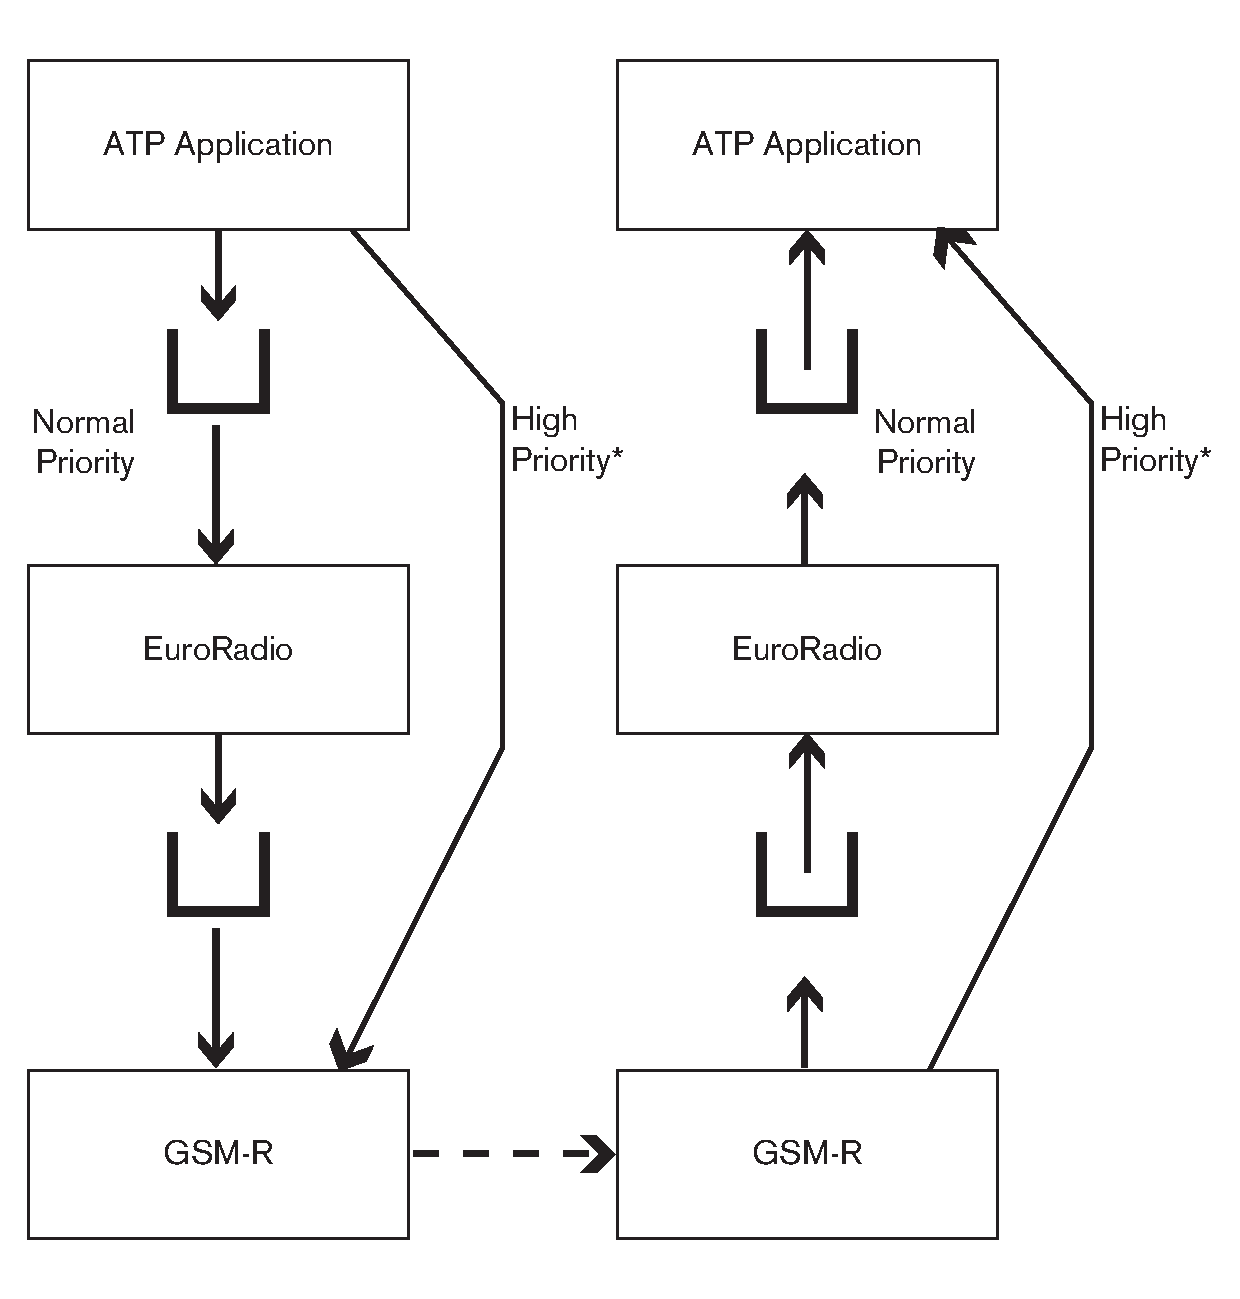
\includegraphics[scale=0.5]{HP-Diagram.pdf}\\
Figure 6.5: \textit{Network Diagram for Normal and High Priority SaPDU traffic}
\end{center}

\subsubsection{High Priority SaPDU Flow}
As demonstrated in the diagram above, when a high-priority message is sent, the message bypasses the queues to EuroRadio and is processed directly to the GSM communications layer for transmission. For clarity, the diagram shows it also bypassing EuroRadio, however, it should be noted that high-priority messages pass through the EuroRadio layer, but do not have any EuroRadio-related information added to the data (header and MAC). Upon arrival of the data to the receiving GSM-layer, it bypasses the queues, and given there is no MAC to authenticate, the High Priority SaPDU is immediately delivered to the Application Layer.

\subsubsection{Permitted Messages and Format}
As discussed in Section 6.7.1, only two messages \citep[Section 8.5.3]{SUBSET-026-8} may be sent as high-priority SaPDUs:
\begin{itemize}[nolistsep]
\item Conditional Emergency Stop -- this contains ``the information of a new stop location, referred to the LRBG" \citep[Section 3.10.2]{SUBSET-026-3}. If the train has already passed the location specified in the emergency stop\footnote{Namely if the end of the train has already been noted as passing the balise group specified}, then it shall proceed, and reject the message from the RBC. If it has not passed the location already, then the ERTMS system will accept the emergency stop, which (if the LRBG referred to in the message is before the end of Authority) will terminate authority at the given location. If the original end of authority in the Movement Authority was set before the location in the emergency stop, the End of Authority (the location where the train must stop) holds.
\item Unconditional Emergency Stop -- when this message is received, the train will `trip immediately', coming to a safe stop. Like conditional emergency stops, a unique identifier to the message is set and only when a revocation of the emergency stop is issued by the RBC, is the train able to enter full supervision mode again, and request a Movement Authority.
\end{itemize}
For both of these messages, any subsequent messages (provided they are not revocations of the standing emergency stop) will be rejected by the train. This includes messages sent by the RBC including Movement Authorities. This means that if an errant emergency stop was issued (possibly for the wrong train), but then a Movement Authority was given, the train must reject that Movement Authority and await instructions from the RBC to restore operational control.

\subsubsection{Threats}
As EuroRadio is the first layer to process data sent over GSM-R, it is the most exposed layer of train-borne ERTMS systems and must deal with a large number of potential threats. Without a MAC in high-priority messages, it is, therefore, possible for an attacker to have broken the A5/1 Cipher in use by the GSM Layer to intercept and interact with train and trackside communications, including train position reports and train clock accuracy, in addition to the ETCS identities of balise groups passed by the train.

With all this data at their disposal, it is therefore possible for an attacker to be able to construct either a conditional or an unconditional stop message and issue it to a train. Whilst this would not impact safety, as there is a safe distance maintained between trains, this would cause considerable delays, given ERTMS would have to recover the state for every train brought to a halt. Network Rail `Delay Minute Costs' are \pounds250 per minute where the cause was their responsibility. Arguably, the ERTMS network and platform is under the control of Network Rail and for a major main-line from London, which is already congested, a single train stopping unexpectedly could cause knock-on delays which could last throughout a day.

A recent time-memory tradeoff attack was presented at ACNS 2015, which demonstrated an attack against the A5/1 Cipher could be completed within nine seconds. Rainbow tables also exist for GSM, which occupies approximately 1.6TB \citep{Karstensen13a} \citep{SRLabs10a} of memory, which, whilst still impractical against current portable computation, could be significantly easier to attack in the future.

\subsubsection{Recommendations}
There is absolutely no sufficient and substantive reason why these messages should not be authenticated. One may suggest that these messages were sent under the pretence that if there was some disaster on the line where the RBC was not capable of performing the cryptographic operations, it should attempt to send a train a stop message regardless. The train should, therefore, assume the worst conditions. This vector, however, can contribute to a number of delays, costing not only Network Rail in the case of the UK, but also other operators in terms of time and cost due to displaced fleet vehicles, staff and other resources.

The solution to this would be to enforce a state where all messages require a MAC to guarantee authenticity, as the GSM layer should not be relied upon to secure communications.\\This has been proven to be broken by a number of researchers, as identified in Section 5.6.

\subsection{Threats to the MAC Algorithm Cryptographically}
At the heart of EuroRadio is the MAC. This authenticates and guarantees to the receiving party that the data being received is genuine and has not been corrupted or modified during transmission. As highlighted in this section, the MAC algorithm uses single DES for chaining all but the last block, which has a triple DES transformation applied. Being derived from the ISO9797 standard means that like GSM-R, it is potentially vulnerable to attacks based on the original ISO standard definition of the MAC. The ISO9797-defined MAC Algorithm Three is used in ePassports \citep{Chothia10a} and in finance applications \citep{IBM}, which have extensive exposure across a number of industries and everyday applications, which are all, therefore, vulnerable to attacks on this standard.

Feix and Thiebauld \citep{MACAlgo3SideChannel} presented a side-channel attack which was able to recover one key used as part of the MAC process. In order to fulfil this attack, the first $n - 1$ blocks are fixed for every MAC produced, where block $n$ is given sufficiently high entropy. For every intermediate ciphertext produced from the DES operation on these $n - 1$ blocks, two guesses are required which can be retrieved using side-channel analysis due to the fact that the resultant $n - 1$ block is XORed with the final block, $n$. Once an attacker has obtained the intermediate state ciphertext and it is known, the first key, K$_1$ may be either guessed or brute-forced, as the attacker has the corresponding plain text and cipher text representations of all blocks up to block $n - 1$. For every guess of the ciphertext, this process would need to be completed twice, once for each bit guessed (0 or 1). The ISO9797-defined MAC algorithm makes use of only two DES operations in the final transformation, with the search space reduced to two guesses, with a further two brute-force attacks on the DES key to retrieve both of the keys used as part of the MAC computation. In EuroRadio, however, three keys are used as part of the DES operations, in encrypt-decrypt-encrypt mode, meaning that this attack presented by Feix and Thiebauld may not be used verbatim as an attack to the MAC algorithm used by EuroRadio.

This attack, however, may still be applied in the context of the $n - 1$ transformations, where we know the plaintext being sent and can produce a MAC forgery as the input to the final 3DES transformation. However, this requires 56 bits of sufficiently random data to be set by the attacker, where the output bits for the MAC would need to be brute-forced to match a genuine MAC following a 3DES operation.

In 1998, Deep Crack, produced by the EFF was able to crack a single-DES key in 56 hours. Today, RIVYERA, the successor to COPACOBANA, a single-DES cracker, is now able to crack DES within a day. Using this premise, an attacker could then establish K$_1$ and create their own MACs in the hope that one may be accepted through a collision attack. This also gives way to identifying the first key used as part of the train key, so future KS$_{MAC_1}$s may be predicted in future communications, if they are able to crack the triple-DES operation using the nonces. With the advances in hardware crackers, this time will continue to reduce.

Using a different process, Biham in 2002 \citep{Biham02a}, presented an attack against single-DES which reduced the overall complexity to a search space of $2^{28}$, and reducing the space for triple-DES key recovery to $2^{84}$ through use of a birthday attack, which looks for key-collisions with $2^{56}$ required plaintexts.

With contextual reference to EuroRadio, it is therefore possible to retrieve K$_1$ through two possibilities - using a side-channel attack as presented by Feix and Thiebauld, or alternatively, the use of a birthday attack where a collision between two MACs is evident. Within the specification for Emergency Stop messages, there is a requirement for the train to acknowledge the command, regardless of whether it is unconditional or conditional. If a \textit{conditional} emergency stop was issued to a train, the corresponding acknowledgement would be sent with a MAC. The emergency stop command could, however, be irrelevant to the train, for example citing a balise it has already passed, or one that does not exist on the line it is using, thus a rejection would be sent. On average, sending $n$ such messages to the train would take approximately $\dfrac{{2^{32.5}}}{{3600 \cdot n}}$ hours to achieve a collision. An attack within a day would require in the order of over 50,000 messages to be sent per second. This would not be possible given the limited bandwidth available to a train, and the likelihood that the volume of messages would overwhelm the GSM-R network. This would result in the train suffering a denial of service attack, which would cause the train to stop, as it would likely reach the end of its Movement Authority with no new messages being received to the EVC.

Once K$_1$ has been established, it is therefore possible to forge messages. One such way is to control the last block of the message being sent, where a valid MAC, $m_p$ for packet $p_1 , ..., p_n$ is known and the attacker wishes to construct a MAC representing $p'_1 , ... , p'_{n'}$. Given that K$_1$ is known to the attacker, he can calculate C$_n$, and set $p'_{n'}$ to be DES$^{-1}_{K_1}$(C$_n$) $ \bigoplus $ (C'$_{n'-1}$). With this, for any plaintext message $p_1,...,p_n$ and $p'_1,...,p'_{n'}$, the corresponding MAC for these messages are the same, $m$.\\
If the last block is not controlled by the attacker, rather it is any other block, $b$ from a message $p_1,...,p_n$ where $1 \leq b < n$, it is possible to achieve another attack. As the full MAC, $m$, will be known to the attacker, they would then work backwards until they have reached the stage where block $b$ would be inserted into the MAC, and perform an XOR to insert the modified message.

Moreover, an attacker who has the plaintext, the corresponding MAC for that plaintext and K$_1$, can brute-force K$_2$ and K$_3$ through a meet-in-the-middle attack, where candidate keys are attempted and once they have been identified for that given MAC, they are validated against other messages sent and their corresponding MACs. This however requires 2 $\cdot$ 2$^{56}$ DES decryption operations and the storage of intermediate results which amounts to storage and memory requirements in the order of petabytes, which is not currently feasible without significant computational cost.

As with any cryptographic algorithm, the relative strength and integrity relies on the strength of its keys. Given that the keys for the MAC algorithm used in EuroRadio are derived using both the train key and the nonces shared by both the train and RBC, the keys are strong and, more importantly, fresh. Thus, the strength of the MAC not only relies on the strength of the three distinct DES keys, but also the nonces sent by the train and RBC, in that they are sufficiently random, or at least appear to be random. On embedded devices, getting sufficient entropy can be an issue, due to their architecture being mainly solid-state with little source of entropy. Rewind time by 10 years, hard-drives and other sensors were good sources of entropy. On a train, this is no different with a number of sources of entropy available, for example using the speed of train wheels, or data arising from the array of sensors onboard. A RBC also has a number of entropy sources available including the number of trains for which it is responsible, in addition to the data retrieved from the interlocking system and other connected systems.

Before a key is formally issued by a KMS for use on an ERTMS entity, posterity checks to confirm that the key is not already in use by another entity under its control, and its relative strength are verified. The ERTMS specifications do not stipulate how key strength is verified in terms of processes and what it deems as `strong'. It is therefore important that, from the outset, the train key is created with appropriate entropy and strength, to allow derivation steps for the session key and any other cryptographic operations to be sufficiently strong. This prevents attacks which are attributed to the use of weak keys. Such attacks include the Diffie-Hellman weak ephemeral key where an attacker could downgrade the HTTPS cipher being used to one that could be broken relatively easy.

The MAC Algorithm used is annotated on the next page, with the modified transformation highlighted.
\clearpage

\begin{center}
 \includegraphics[scale=0.5]{ModMacAlgo3.eps}\\
Figure 6.5: \textit{Schematic of Modified MAC Algorithm Three, used in EuroRadio}
\end{center}

\subsubsection{Recommendations}
When a train reaches the limit of responsibility offered by a RBC, a handover process takes place where the train is accepted into the next RBCs area of responsibility. It is here that the EuroRadio session is terminated and a new one established with the accepting RBC \citep[Section 3.15.1.3]{SUBSET-026-3}. It is this requirement to establish a new session during handover which means that we should not have concerns over the use of long-term keys, as session keys will only be in use for a short amount of time. On a high-speed line, this is not feasible for exploitation by an attacker. However, at major intersections where main-lines meet, for example, or on the approach to termini, where a train may cross a number of lines to reach its terminal platform, the attacker model is made very real, simply because a train will be connected to the GSM-R mast for a longer period of time, and, when on approach, may be travelling at a low speed\footnote{Birmingham New Street has an approach speed of 10mph \citep{NetworkRail15f}}.

The vulnerabilities discussed above do pose a significant threat to EuroRadio and the solutions, whilst they may appear minor, would make this protocol layer significantly more secure. Measures such as using triple-DES in the first and last block transformations would prevent a length extension attack, given an attacker cannot predict the intermediate states as easily, based on the first transformation. This prevents a side-channel attack directly as an attacker would have to establish the 3DES key before being able to forge their own MAC, something that, by today's current standards, is not feasible. Likewise, the time taken to break a triple-DES key is still infeasible by modern standards, so would delay an attacker from forging valid messages.

That, however, does not mean that the use of triple-DES is the only solution. Current estimates place triple-DES as being hardy through to 2030 \citep{NIST12a}, however for a long-term next-generation system which will far exceed this date, it is critical that a stronger MAC algorithm is available. The Advanced Encryption Standard (AES) encryption scheme is known to be strong even at 128 bit lengths, and, using this, would be an appropriate consideration. This, however, would require changes to software, given the MAC, nonce, Session Keys and `Seeding Keys' are 64 or 192 bits respectively in length. Doubling the size would not impact the storage of keys and the MAC would be sufficiently strong to prevent an attack, due to the increased entropy and inherent strength of AES that it currently holds. Moreover, AES can be implemented in hardware, and is typically now part of instruction sets on CPUs, meaning that there would be little impact overall in using these operations.

In addition, to prevent replay, deletion and incorrectly sequenced messages at this level of the stack would simply require a sequence number. TCP uses 2 bytes (16 bits) where the maximum value accepted is 65535 prior to wraparound. For trains, which may be parked or preparing to shunt for an extended amount of time, this could result in wraparound, where an attacker waits and replays a message at the right time -- thus a longer sequence number value, of 4 bytes would be recommended.

Another interim solution to prevent length-extension attacks to which the MAC algorithm is vulnerable is to also perform a 3DES transformation to the first block, as this means that a side-channel attack is not directly possible. This is because an attacker would have to establish the 3DES key before being able to forge their own MAC, something by today's current standards is not feasible.

\subsubsection{Impact to Implement Security Improvements}
As previously identified, single changes can significantly improve the security of ERTMS. Given the computational power now available for general use and embedded devices, there is no reason why established and formally proven forms of cryptography cannot be used in the generation of a MAC with respect to high-priority messages. In an experiment of 1 million rounds of generating a high-priority message and then performing a MAC operation, the results were modelled in \textsf{R}, removing outliers $\pm$ two standard deviations from the mean, and analysing them shown in the following table:\\
\vspace{-0.5cm}
\begin{center}
\begin{longtable}{|c|c|c|}

\hline \multicolumn{1}{|c|}{\textbf{Measurement}} & \multicolumn{1}{c|}{\textbf{Time to generate HP SaPDU}} & \multicolumn{1}{c|}{\textbf{Generate + MAC HP SaPDU}}  \\ \hline \hline
\endfirsthead

\multicolumn{3}{c}%
{{\bfseries Time Measurements -- continued from previous page}} \\
\hline \multicolumn{1}{|c|}{\textbf{Measurement}} & \multicolumn{1}{c|}{\textbf{Time to generate HP SaPDU}} & \multicolumn{1}{c|}{\textbf{Generate + MAC HP SaPDU}}\\ \hline \hline
\endhead

\multicolumn{3}{|r|}{{Continued on next page}} \\ \hline
\endfoot

\hline \hline
\endlastfoot

Valid Samples & 932,015 & 935,455 \\ \hline
Minimum & 331ns & 1,354ns \\ \hline
Maximum & 395ns & 1,354ns \\ \hline
Average & 355.545ns & 1,417.757ns \\ \hline
Standard Deviation (s) & 13.123ns & 38.169ns \\ \hline
Overall Impact & 1x & 3.988x \\% \hline

\end{longtable}
\end{center}
\begin{center}
\vspace{-1.0cm}
Table 6.6: \textit{Summary of measurements taken to assess impact of employing EuroRadio protection to protect HP SaPDUs}
\end{center}

Overall, whilst performing the necessary MAC operations introduces a delay in message generation times by a factor of approximately eight, which is a very small number especially when working in terms of nanoseconds (when one considers the impact of also verifying the MAC at the receiving end), the benefits far outweigh the negligible delay impact. As a safety-critical feature in ERTMS, it is considered a wholly acceptable delay. It should be noted that these values were calculated on a computer with an Intel$^{\textregistered}$ Core i5 quad-core processor operating at 3.2GHz. To see any noticeable difference in time values requires a resolution of is 1 x 10$^{-9}$ seconds, meaning that in a production system which may have lower computing power available, the worst case delay will remain in terms of micro-seconds (1 x 10$^{-6}$) or milliseconds (1 x 10$^{-3}$). This delay would therefore be minimal, and not impact safe operation of the train. The accompanying histograms generated by R are detailed in Appendix Two.

\subsection{Implementing Improvements to the EuroRadio Layer}
As EuroRadio is implemented in software and not hardware, it is appropriate that any changes to improve and strengthen its role are also implemented in software. Within the ERTMS design is a future-proof method of ensuring it meets the needs and demands globally through new system revisions. At present, when new versions of the ERTMS system are rolled out to rolling stock, there is a requirement to be able to support backward-compatibility, as national deployment of the new ERTMS version may take time. There is allowance for up to three sequential versions to be in operation at the same time, with an option for a fourth, should there be a national phase-out.

The proposed solutions of implementing a sequence number, can be included as part of the EuroRadio specification and rolled out within a new ERTMS version. The cost to suppliers, Rolling Stock Operating Companies (ROSCOs) and manufacturers is therefore static, where a new version can be rolled out as part of scheduled maintenance to a train. The alternative, where hardware may be required would have an unpredictable and potentially unacceptable cost, dependent on the amount of equipment that requires to be upgraded, either train-borne or track-side.

Most CPUs today support the AES instruction set, so with the MAC using the AES-128 algorithm, this change could be leveraged in code, meaning that not only does the impact on performance become minimal but also the fix would lie purely in software, with no further equipment required.

A short-term fix of applying a 3DES transformation to the first block in addition to the last block, as defined to the MAC algorithm, has therefore, negligible effect in generation times, as the transformation is only taking place in two of $n$ possible blocks, but would vastly reduce the possibility of an attacker attempting to break K$_1$ and use it to create a MAC which would be rendered valid upon receipt.

\subsection{Closing Remarks}
EuroRadio takes what should now be considered an open communications layer (GSM-R) and attempts to make it partially secure by ensuring authenticity and integrity of messages passed to it. The session key itself is good, where a new one is generated per EuroRadio session, which is guaranteed to be fresh and each entity has mutual belief in the key. The key itself is exclusive in the way that only one train and a given set of nonces will produce that 3DES key, which gives a good key. Entities are appropriately verified with specific actions once authenticated with a far-end operative.

However, the MAC Algorithm used by EuroRadio is weak, which, whilst not currently exploitable, will be exploitable within the next decade or two and could lead to a state where the integrity of ERTMS is compromised. In addition, the basic principles of an effective secure protocol are non-existent, for example replay and deletion, where EuroRadio should not leave it to the Application Layer to provide sufficient protection against these threats. Critically, the decision to provide high-priority messages without adequate integrity and authenticity checks is not acceptable and could do more harm than the benefits it provides.

\clearpage

\section{Application Layer}
\subsection{Overview}
Dependent on the ERTMS entity in use, the upper layer from EuroRadio varies. On a rail vehicle, the EuroRadio layer feeds immediately into the ATP Application Layer, which has a number of assumptions placed upon it from the EuroRadio layer. In RBC $\leftrightarrow$ RBC communications, however, there is an additional layer, the Safe Application Interface (SAI) which is responsible for some of the defences which the Application Layer in Train $\leftrightarrow$ RBC communications would otherwise perform.

For the threats that EuroRadio is unable to provide protection against, it is the Application Layer which must `fill the gaps' in order to be compliant with EN50159. One could consider this an area of concern, where two layers are responsible for providing overall security to a safety-critical platform. To illustrate this, the threat/defence matrix from Section 6.3.2 has been expanded to include the defences that the Application Layer offers in addition to EuroRadio. Together, these two layers are able to fulfil the requirements of EN50159 and are therefore compliant for use on rail applications.

\vspace{-0.5cm}
\begin{center}
\begin{longtable}{|c|c|c|}

\hline \multicolumn{1}{|c|}{\textbf{Threat}} & \multicolumn{1}{c|}{\textbf{EuroRadio}} & \multicolumn{1}{c|}{\textbf{ATP Application Layer}}  \\ \hline \hline
\endfirsthead

\multicolumn{3}{c}%
{{\bfseries Threat/Defence Matrix -- continued from previous page}} \\
\hline \multicolumn{1}{|c|}{\textbf{Threat}} & \multicolumn{1}{c|}{\textbf{EuroRadio}} & \multicolumn{1}{c|}{\textbf{ATP Application Layer}}\\ \hline \hline
\endhead

\multicolumn{3}{|r|}{{Continued on next page}} \\ \hline
\endfoot

\hline \hline
\endlastfoot

Repetition & $\times$ & \checkmark \\ \hline
Deletion & $\times$ & \checkmark \\ \hline
Insertion & \checkmark & $\times$ \\ \hline
Re-sequencing & $\times$ & \checkmark \\ \hline
Corruption & \checkmark & $\times$ \\ \hline
Delay & $\times$ & \checkmark \\ \hline
Masquerade & \checkmark & $\times$ \\% \hline

\end{longtable}
\end{center}
\begin{center}
\vspace{-1.0cm}
Table 7.1: \textit{Threat/Defence Matrix for EuroRadio and the Application Layer, measured against EN50159}
\end{center}

\subsection{Application Layer in Detail}
The Application Layer does not just provide additional measures for security - it should be considered as an interface to the train API for EuroRadio. It is this layer which interfaces with the local ERTMS application, and from which data is first transmitted and finally received.

\subsubsection{Assumptions Placed on the Application Layer}
As shown above, what EuroRadio does not defend against must be prevented by the Application Layer. Given that authentication and integrity has been `guaranteed' by the EuroRadio layer, cryptography is unsuitable for these checks, as it does not provide any additional defences. Instead, the Application Layer uses a time-stamp relative to the train time, occupying 32 bits, with 10ms precision. To achieve a wraparound to a zero value would take approximately 497 days \citep[Section 7.5.1.154]{SUBSET-026-7}. The time-stamp, therefore, is simply a virtual reference to time from some artificial zero-point, and not say, the Unix time. In an analysis by Gradowski et al \citep{Gradowski14a}, when a RBC needs to send a message, it is required to ``measure the time... which has passed since the last received message from the train" to send a valid time-stamp. These time-stamps are used solely for the purpose of detecting whether a message has arrived out of sequence or replayed, as the time-stamp of the message received must be greater than the time-stamp of the last received message \citep{Ansaldo05a}.

To cope with possible issues of time delay, the train and RBC calculate an acceptable amount of time before messages should time out, prior to assuming they have not been received and resending them. The specifications also stipulate what should happen after a period of inactivity. However, these are specified as national values by the operating countries, and may be one of three values - one which trips the emergency stop on a train, one which applies the train brakes and the other has no reaction whatsoever \citep{RSSB12a}. Whilst this applies only to a timeout in the general sense where ``no safe message has been received from the track" \citep[p. 81]{SUBSET-026-7}, this timeout may be set between 0 and 254 seconds. Similarly, it is also possible to set all bits in the 1 byte block to zero, indicating an infinite amount of time (i.e. there is no timeout).
\subsubsection{Key Messages}
All messages for the Application Layer follow a set format, where optional data and packets are given which feature the different variables required for that message. The figure below demonstrates the general `packet' structure and features.

\begin{center}
 \includegraphics[scale=0.4]{TrainAppMessageFormat.eps}\\
Figure 7.2: \textit{Generic Message Format for Application Layer Messages between Train $\leftrightarrow$ Track in each direction}
\end{center}

The following messages are of paricular interest, given they contain sufficient entropy and are vital to the safety-critical aspect of ERTMS:\\
Train $\rightarrow$ Track:
\begin{itemize}[nolistsep]
\item Train Position Report (Message 136)
\item Acknowledgement (Message 146)
\item Acknowledgement of Emergency Stop (Message 147)
\item End of Mission (Message 150)
\end{itemize}
Track $\rightarrow$ Train:
\begin{itemize}[nolistsep]
\item Movement Authority (Message 3)
\item Conditional Emergency Stop (Message 15)
\item Revocation of Emergency Stop (Message 18)
\item Train Accepted (Message 41)
\end{itemize}
The significance of these messages is explored further below.\\
Train Position Reports additionally contain the precise location of a train, in relation to a specific balise group passed. This allows the ERTMS system to know the location of the train precisely and inform the next interlocking decision. This particular type of message also contains the train-borne time, train ETCS ID and potentially optional packets which contain non-ERTMS related data, outside of the core specification.

Message Acknowledgements contain no position report, rather they contain the train-borne time, ETCS ID and the time-stamp contained in the message to be acknowledged\footnote{Currently, ERTMS messages have no concept of sequence numbers, and the assumption is that no two messages are sent with the same time-stamp.}. Acknowledgements of emergency stops, however, have a slightly different structure, which only contains only the train-borne time, ETCS ID, and additionally, the numerical value of the emergency message which is to be acknowledged and a value, \texttt{Q\_EMERGENCYSTOP}, which cites whether the command has been accepted or not. If the command has been accepted, the End of Authority (the limit of the current Movement Authority) either remains the same or is shortened (based on what the conditional stop indicates). If a command were to be rejected, this is either because it is `not relevant' \citep[p. 70]{SUBSET-026-7}, due to an unconditional emergency stop being issued, or if the location specified in the conditional emergency stop has already been passed by the train.

The `End of Mission' message simply tells the RBC that the journey has been completed and takes the same structure as a Train Position Report, with the train-borne time and train ETCS ID, with the train position either relative to a single, or double balise group included. It does not, however, contain any optional data, which the position report could contain.\\\\
Messages delivered through trackside communications to a train are typically larger in size but fewer in number compared to messages sent by a train.

Movement Authorities are one such example. These contain the train-borne time, a flag indicating if the authority must be acknowledged or not, as well as the identity of the last relevant balise group. These are then accompanied by `Packet 15' which contains the full Movement Authority information required by a train, including features like direction of travel, permitted speed at the limit of authority, length of section in that authority, validity times and danger point information\footnote{This may be included if there is a train outside of the authority limits, as this packet is also proposed for use in ERTMS Level 3.}. Optional packets may be included, which again are data packets outside of the ERTMS specification scope.

Conditional Emergency Stops contain the train-borne time, whether the command must be acknowledged, the ID of the LRBG being used as a reference location, an identifier for this particular message and a scale defining a measurement of distance in metres. Using this scale, the distance from the specified LRBG indicates where the stop is effective and in which direction. The train uses this information to identify if the message is applicable or not.

Revoking an emergency stop message is simple - it contains the train-borne time, a flag to signify whether an acknowledgement is required, the ID of the LRBG and the identification number of the emergency stop message. Thus, a RBC must revoke a specific message in order for the ERTMS system to `reset' and for the appropriate recovery procedures to be allowed.

Train Accepted messages are sent following a request by a train to be supervised. This message contains only the train-borne time, whether an acknowledgement is required and the ID of the balise group submitted by the train.

RBCs and trackside elements are not required to acknowledge messages sent to it by a train with an explicit `acknowledgement' message. The `API' instead is designed in a way that when a message is sent by a train to a track-side element, it receives a response with a corresponding message, which may be interpreted as an acknowledgement.

\subsection{Safe Application Interface (SAI) Sublayer}
Within the definition of RBC $\leftrightarrow$ RBC Handover of a train, there is another intermediate layer between EuroRadio and the Application Layer. This has its own protection which meets the requirements of EN50159, where the Application Layer may be implemented differently to Train $\leftrightarrow$ Track communications. This is understandable, given RBC entities are connected by fixed network, resulting in a more reliable and predictable network connection.

\subsubsection{Defences Offered by the SAI Sublayer}
The SAI layer adds a header to Application Data before being passed to the EuroRadio layer. The EuroRadio layer remains unchanged when compared to the train-borne counterpart. This layer offers protection against repetition, deletion and resequencing through the use of a 2 byte sequence number \citep[p. 21]{SUBSET-098}, with a ``delay defence technique" \citep[p. 15]{SUBSET-098} which comes in the form of either a triple time-stamp or an execution cycle counter.

The technique of using sequence numbers is similar to the process used in the TCP protocol, where each party participating in the connection sets its own random value $r \in 0 \leq r \leq 65536$. Although the first sequence number sent is not checked, any message subsequently received is verified against this value. When the maximum value allowed is reached, the sequence number will wrap around to be zero. If there is a `gap' between sequence number values, it should be considered that a fault occurred. The SAI maintains a count of how many of these errors are allowed, either due to repetition, deletion or re-sequencing. If it reaches a certain set threshold, the connection will be released. This value is set nationally as T$_{succ\_err}$ \citep[Section 5.4.10]{SUBSET-098}.

Immediately after the EuroRadio connection protocol completes, the triple time-stamp or execution cycle counters are initialised. A triple time-stamp and execution cycle counter is used to detect delays in transmission. However, the sequence counter is only able to detect sequencing errors, including deletion and replay.

A triple time-stamp (TTT) is formed of three 4 byte values (approximately 497 days, measured in a resolution of 10ms), with execution cycle counters also 4 bytes. Triple time-stamps are defined by the clock-offset computations between sender and receiver. In order to agree on the time-stamp (as times are based on the train clock), an initialisation procedure is followed to allow a suitable offset to be estimated. Each time-stamp serves a unique purpose, namely the first contains the sender time-stamp at time of transmission, with the second being the time-stamp of the last message sent to recipient by the current sender. The final time-stamp is the time-stamp of the last message sent by the current sender. These together not only help identify `jitter' in the communications, but if implemented, could also identify whether a message has been replayed at a later time or injected, because both parties have a direct relationship for communications and a means of proving when messages were sent. Triple time-stamping makes no assumptions regarding transmission and compute cycles, where the second and third time-stamps are used to perform a `rolling update' of the offsets, with the first being used to compute validity and identify potential delays. A regular procedure to recalculate offsets is also required.

This method of defence requires five messages to be sent prior to data being sent, where the first and second messages allow the time-stamps to be synchronised between parties. These are accepted regardless of their values but in the third step, the offset is established.  When the recipient receives a message, it validates the sender time-stamp, and applies a formula to allow some offset and extra delay, again a rolling process. If a delay is detected, the message is discarded, and error handling is left to the system implementer.

Execution Cycles (EC) work differently to the triple time-stamp, where in the SAI header, the time-stamps are set to zero, and appended with a 4 byte counter. In this method, each party has an expected value as time progresses. Each party has an independent counter, where, upon receipt of an EC value, validates whether it is a value which was expected. Compared to triple time-stamping, the initialisation process has fewer steps, where a period is specified as part of the initialisation, with a resolution of 1ms. At each cycle of the receiver, the expected EC value used is updated with some ratio defined using the period and an offset. If no message is received in a set EC, then the receiver computes this delta value, otherwise if more than one message is received in a cycle, the most recent value is used.

This method of protection should ideally be employed on Train $\leftrightarrow$ Trackside communications, as it is a potentially effective way of detecting delays with appropriate proof that there is no `foul-play' in the connection.

\clearpage

\section{Other Features of ERTMS Investigated}
\subsection{Key Management}
\subsubsection{Overview}
ERTMS has a strong reliance on cryptography, which uses secret keys to protect data. These keys are unique to the ERTMS entity, where each country will have its own Key Management System (KMS). At any one point, no KMS may act as the Key Management Centre (KMC) for more than one country. At the start of the project, whilst looking at ERTMS as an entire platform, this area was investigated further to establish how keys are used.

\subsubsection{ERTMS Key Management Hierarchy}
In ERTMS, the Key Management Centre is core to the operation of the entire platform, where entities need to communicate using secret keys as part of the proof of integrity in messages. Key Management Centres may be connected to other centres, say the UK KMC may be operated by the Infrastructure Manager responsible for the UK, and may be contactable by the KMC for Germany. This allows seamless interoperability throughout these rail networks. However, a KMC which is not in the home domain cannot issue keys to other KMCs -- these KMCs must make requests only to the home KMC.

Within this hierarchy, the KMC is formed of servers and clients, with ETCS entities as an external user. Servers organise the overall key management process, generating and validating keys, which are stored securely for both home and foreign managed entities. In addition, these servers are responsible for key distribution and maintaining their state, initiating key management tasks, for example, updating the validity of a key where required. When this takes place, requests to ETCS entities are generated to either update, install or delete the keys and liaising with foreign KMCs where required. When a key is issued, it monitors the installation and confirmations to track if the key has been installed. As seen in typical servers, the KMC server maintains archives of keys, as well as logs for the purposes of auditing \citep{KPMG13a}.

There is no hierarchy of KMCs themselves -- they sit at the same level, where there is no KMC which represents Europe, for example. Likewise, only one KMC is authoritative, where all key management tasks for entities are performed at that KMC - no other KMC may perform these actions.

Clients act as the interface to the KMC, where key management actions may be requested, and are the point at which keys may be retrieved. It is the KMC Client which reads the status of the keys and confirms the installation status of these keys on the appropriate entity.

ERTMS entities are not part of the KMC network, where there may be a physical airgap between the KMC and the entity on which the key is to be installed. These entities receive the keys and either install the keys on the ETCS on-board unit (OBU), or the trackside equipment, for example the RBCs. These entities will use the keys provided according to their validity and will update and/or delete the key when requested.

One element that is not defined precisely in the operational guidelines for ERTMS is whether a train is able to start a mission or proceed with an expired key, or one which could expire during a journey. It is considered that this should be immediately addressed and the specification clarified such that if a train is travelling with a revoked or expired key, it should not be accepted by a RBC and refused safe supervision.

\subsubsection{Keys Used in ERTMS}
Depending on the type of communication in use, different cryptographic keys are used for those transmissions. In ERTMS, the current matrix \citep[p. 15]{SUBSET-038} for keys used is below:


\vspace{-0.5cm}
\begin{center}
\begin{longtable}{|c|c|c|c|}

\hline \multicolumn{1}{|c|}{\textbf{ERTMS Entities}} & \multicolumn{1}{c|}{\textbf{I\&A}}  & \multicolumn{1}{c|}{\textbf{Message Authentication}}  & \multicolumn{1}{c|}{\textbf{Encryption}} \\ \hline \hline
\endfirsthead

\multicolumn{4}{c}%
{{\bfseries Threat/Defence Matrix -- continued from previous page}} \\
\hline \multicolumn{1}{|c|}{\textbf{Threat}} & \multicolumn{1}{c|}{\textbf{EuroRadio}} & \multicolumn{1}{c|}{\textbf{EuroRadio}}  & \multicolumn{1}{c|}{\textbf{EuroRadio}}  \\ \hline \hline
\endhead

\multicolumn{4}{|r|}{{Continued on next page}} \\ \hline
\endfoot

\hline \hline
\endlastfoot

Train $\leftrightarrow$ RBC & K$_{MAC}$ & KS$_{MAC}$ & $\times$ \\ \hline
RBC $\leftrightarrow$ RBC & K$_{MAC}$ & KS$_{MAC}$ & $\times$ \\ \hline
KMC $\leftrightarrow$ RBC/Train & $\times$ & K$_{TRANS_1}$ &  K$_{TRANS_2}$ \\ \hline
KMC $\leftrightarrow$ KMC & $\times$ &  K$_{KMC_1}$ &  K$_{KMC_2}$

\end{longtable}
\end{center}
\begin{center}
\vspace{-1.0cm}
Table 8.1: \textit{Threat/Defence Matrix for EuroRadio and the Application Layer, against EN50159}
\end{center}

\subsubsection{Inserting Keys on ERTMS Entities}
When a train is first produced, a KMC generates a key for the train, which is signed and encrypted before being given to the train. The train and KMC share a unique key which is used to validate the key being transferred and another key to encrypt the payload, to ensure full secrecy. If the media that was used to transport the keys were to be compromised, then the keys remains secure.

This is crucial to ensure that the safety and integrity of ERTMS remains intact, as the keys for KMCs and potentially RBCs may be valid for a number of years. Manufacturers such as Siemens and Alstom should install new keys as per maintenance schedules.

Key management, however, gets complex when trains are crossing international borders. The train key is shared with neighbouring KMCs in the region that the train may travel through so that it can be accepted by RBCs in that domain. It is the responsibility of the home KMC to generate the key for trains and other ERTMS entities. RBCs never allow keys to be distributed outside of their home domain.

\subsubsection{Key Derivation Used in EuroRadio}
To establish and authenticate a EuroRadio connection between ERTMS entities, a session key (for symmetric encryption) is used which is negotiated between the two connecting entities. A long-term key, $K_{MAC}$ is stored on the track-side ERTMS entity and distributed to RBCs by the Key Management Centre (KMC). The premise of key distribution to RBCs is that if a train were to come into an `area of responsibility' covered by a RBC, it must then hold the key to enable communication.

The two random nonces, $R_{RBC}$ and $R_T$ are used as part of the key derivation as follows:\\
\begin{algorithm}[H]
\floatname{algorithm}{Key Derivation}
\renewcommand{\thealgorithm}{}
\caption{Calculation of a session key to authenticate messages between ERTMS entities}
$R_T$: Train Nonce, $R_{RBC}$: Radio Block Centre Nonce, $K_{MAC}$: Train Key, $KS_{MAC}$: Session Key\\
\textit{Let $K_{MAC}$ = $(K_1,K_2,K_3)$.}
%\vspace{-0.5cm}

\label{Key Derivation}
\begin{algorithmic}[1]
\STATE Let $R_{T}$ = $R_T^L$ $\mid\mid$ $R_T^R$
\STATE Let $R_{RBC}$ = $R_{RBC}^L \mid\mid R_{RBC}^R$
\STATE $K_{S1} := DES(K_3, DES^{-1}(K_2, DES(K_1, R_T^L \mid\mid R_{RBC}^L))). $
\STATE $K_{S2} := DES(K_3, DES^{-1}(K_2, DES(K_1, R_T^R \mid\mid R_{RBC}^R))). $
\STATE $K_{S3} := DES(K_1, DES^{-1}(K_2, DES(K_3, R_T^L \mid\mid R_{RBC}^L))). $
\STATE Let $KS_{MAC} = (K_{S1},K_{S2},K_{S3})$.

\end{algorithmic}
$\Rightarrow$ \textit{Session Key Established}
\end{algorithm}
\begin{center}
\vspace{-0.4cm}
Figure 8.2: \textit{Key Derivation for a EuroRadio Connection}
\end{center}

$K_{MAC}$ is a 192 bit triple key, which is used in the Encrypt-Decrypt-Encrypt (EDE) 3DES mode to establish the session key. Note, for $K_{S3}$, the left-most halves of the nonces are reused, but the keys used for the EDE process are used in a different order to ensure that $K_{S1} \neq K_{S3}$ which would result in only two distinct keys being produced, reducing 3DES to double-DES.

\subsection{ERTMS Versioning}
Given the widespread deployment of ERTMS across many nations, making changes is not as simple as running one single version on the network. Trains will inevitably be upgraded against different schedules to newer versions of the ERTMS system and application, and, at all times, interoperability must remain. For this reason, ERTMS is designed to allow three active versions of the ERTMS system to operate, with provision for a fourth during phase-out to ensure full compatibility \citep{SUBSET-104}. This potentially means that issues found in the ERTMS specification need to be introduced in future versions, rather than patched in previous versions, maintaining consistency throughout. This would be an opportunity where the phase-out option would be used to maintain interoperability whilst the upgrade takes place.

Additionally, as ERTMS is a co-operational effort by large corporations like Siemens, Alstom, Bombardier and Ansaldo STS, their equipment and systems require consistent patching, otherwise their platforms are at risk of not being ERTMS-compliant and could result in incompatibility, especially where a train transitions from one ERTMS system to another\footnote{For example from a Siemens L2 installation to Ansaldo STS L2 system}.

\subsection{ERTMS as an Industrial Control System}
\begin{center}
 \includegraphics[scale=0.5]{ERTMSPrezi.eps}\\
Figure 8.3: \textit{Derived hierarchy of ERTMS}
\end{center}
At the start of the project, I considered ERTMS as a network of interconnected systems and produced a diagram, which demonstrated each link.

After scrutinising the ERTMS specifications, the diagram was further developed as shown above, to show where, for ERTMS, data may traverse, and the key actions that each entity performs in the platform.

Crucially, this analysis highlighted possible vectors for attacks, such as incorrect EuroBalise data which could propagate to the RBC and result in an incorrect decision. In ERTMS/ETCS Level 3, this is most critical, as they are the only reliable source of location data. Likewise, the Regional Control Centres receive data from RBCs to manage the overall state of the railway network. This data needs to be reliable and accurate to prevent potential human error.

Key to the operation of ERTMS is the Key Management Centre, where, if an invalid key was issued, or leaked, the integrity and security of ERTMS could be critically compromised.

To date, no other researcher or security expert has identified the potential for those attacks presented in this project, nor have other authors acknowledged their gravity.

The attacks presented in this paper are very real, and depending on how GSM-R allows routing, it may be possible to affect the entire rail network.
\clearpage

\section{Other Research in this Domain}
To gain a more comprehensive picture for further research into ERTMS in railway applications, I read and reviewed an extensive range of papers. Based on my overall assessment, my conclusion was to focus on the security of the train to track communications link, as this is the most obvious area to attack by cyber-criminals.
\subsection{Research into ERTMS}
Different approaches are used to provide a formal analysis and proof of security of ERTMS at various levels. These present different ways of understanding ERTMS in specific areas.

Franekova et al presented a safety analysis of the cryptographic mechanisms used in {GSM-R} in 2011, using the UML methodology to demonstrate a birthday attack on the DES encryption algorithm \citep{Franekova11a}. References are made to the ERTMS model being implemented as an OSI-style stack, with the addition of the EuroRadio layer between the Communications and Application Layers.

It was this paper which exposed EuroRadio to me for the first time in my analysis of the overall security of ERTMS and gave an outline of some of the ERTMS components. The reference structure of a message was, however, confusing, as a train does not have the Adaptation or SAI layers in the stack, rather it is only for RBC to RBC communication.

Of particular interest from this paper is the use of UML to implement a model of the attack, where $2\cdot2^{28}$ memory allocations would be required with the same amount of encryptions to find the possible keys in use. Their attack used a fairly low-powered computer by modern standards, with approximately $^{1}/_{4}$ of the normative power today. The results claim the average time taken in the worst case as 2$^{15}$ realisations in just one second.\\
The proposals from Franekova touch on some the recommendations drawn from this project paper, such as where a more cryptographically secure cipher such as AES could be deployed, however, the required changes are very different. In their research paper, the changes simply increase the block size to 128 bits, and retain the 192 3DES key, but use 128 bits of that key for the AES encrypt operations. This reduces the need to reissue keys, however it does leave 64 bits of key not being used. This is understandable in the context of interoperability, where another country may use the modified MAC algorithm as the safety option. However, this notion of mismatched key length and cipher length should be phased out, where the key length must match the cipher length \citep{Garcia13}. An alternative proposal, however, changes the mode of the final transformation from EDE to EED. Given 3DES is only approved by NIST for use through to 2030, this would only be another short-term solution to a long-term problem.

UML appears to be a common way for formal verification of a protocol or system, rather than using formal tools like Proverif and experimentation to report results. Zhang et al during 2011 used UML and translated it into a model which the SPIN verifier could use and were able to report a sequence of transitions where a state of deadlock was achieved \citep{Yan11a}. Like other papers explored below, the researchers used the state machine of EuroRadio to create a model which captures all possible states, including idle, data and disconnected states. Their trace of the deadlock is of importance, as a safety-critical protocol should never be in a position where it is possible to achieve a state where there are no remaining state transitions.

In contrast, Rosaria et al \citep{Ansaldo05a} performed an analysis using UML some six years prior to Franekova and Zhang. The focus of their paper was to assess and quantify EuroRadio against EN50159 and use UML to model it. As discussed earlier in this project report, GSM-R is not able to offer certain guarantees and it is the responsibility of the EuroRadio layer to provide guarantees for safety. From this analysis, the team were able to discover areas of deadlock, intolerances to failure, and contradictions between sections of the FIS document for EuroRadio, which could lead to ``an unsafe state". This raises serious concern on the ERTMS ratification and improvement processes, as one would have thought that six years would be an acceptable period to introduce appropriate changes, especially as ERTMS gains traction and adoption as the national solution in later years.

During 2013, Cecchetti et al introduced an implementation to ERTMS/ETCS Level 1 of the Radio Infill Unit (RIU) \citep{Cecchetti13a}, which allows a train to receive a Movement Authority a set distance ahead of a signal, which resolves the `chasing signals' issue faced in the UK rail network. The paper highlights the critical points regarding ATP and how the infill units would operate, as well as some background on ERTMS. The notion of a train API is introduced which refers to the Application Layer, as well as the elements which make up ERTMS as an industrial control system, with discussions on their contribution, and infill deployment. Figure 8 of the paper shows the stack bypass used by high-priority messages, but does not make it explicit in how it bypasses the verifications, clarified in Figure 6.5 of this paper, to show how there is no integrity of authenticity validation carried out.

An alternative form of analysis through Petri Net was devised by Hongjie et al during the same year. Rather than using a UML model to verify the protocol, they use the notion of petri nets, modelling the state machine of EuroRadio and all possible transitions from there \citep{Hongjie13a}. In this model, they were able to provide a statistical analysis rather than a formal analysis, simulating and measuring the performance of the protocol, assessing fault tolerance and how the protocol handles factors which could otherwise influence it. This however has more application to security analysis, but does demonstrate other research in this area.

None of these papers, however, highlight the potential areas vulnerable to attack identified by this specific research project, whereby an attacker is able to successfully forge emergency stop messages and, using modern apparatus, is also able to establish K$_1$. In addition, there is no mention of existing threats to the A5/1 cipher being applied to ERTMS, which allows an attacker to be far more damaging.

\subsection{Key Management}
As identified previously in this paper, Key Management will be a major operational issue following the successful national introduction of ERTMS. Management of keys will become a challenging task, especially when coupled with the concept of interoperability, where the KMS will also have to deal with keys generated by a foreign organisation. The solution to this is to employ online key management, where a patent on a `Method for ETCS Online Key Management' on behalf of Siemens was granted in Germany \citep{SiemensPatent}.

This patent allows RBCs to retrieve keys from the KMC via `a data link' rather than being given the keys in advance, where the train may instead enter a RBC area of responsibility it has not previously entered. At present, the only online element for Key Management is foreign key handover, where one KMC may request a particular key from another and vice versa to ensure interoperability. This may also be performed offline, however, this restricts the potential interoperability of the rail network. The patent awarded to Siemens does include a `Personalization Key' which allows transport of train keys by the manufacturer on their systems using proprietary means. This limits the freedom that current ERTMS key management offers and introduces a possible attack vector, where the vendor may suffer a security breach and the key is divulged.

It is understandable that a train manufacturer may wish to have a key in order to load the train key onto the train. The Key Management Centre could however double-encrypt the key with the inner encryption being performed with a key only the KMC and train possess, and the outer encryption with a KMC - Manufacturer shared key. Thus, if there were a compromise, the integrity of the train keys would remain intact, as they are encrypted with a key only the train and KMC may use. With this proposed solution, there is a fail-safe measure where, should any one of external parties be compromised, the key would remain secure. This raises a question about how the key should be stored on the train -- a device like a TPM would protect the integrity of the key, however, this would require research.

Instead, if the protocol used for KMC $\leftrightarrow$ RBC were formally proven, RBCs and trains could employ the same protocol, where the KMC generates a key to demonstrate proof of knowledge to the entities. This, however, would require modifications to the EuroRadio protocol to ensure that changes made at key-level were made to improve, and not detract from the existing security properties that protocols may guarantee.
\clearpage
\subsection{Secure MAC Algorithms}
In 2004, Handschuh and Preneel wrote an article, aptly named `Minding Your MAC Algorithms?' \citep{MACAlgos04a}, which gives some background to why MACs are important to security, namely that they prevent forgery, forcing an attacker to perform ``an exhaustive key search". It makes a number of recommendations for production systems, which may be assessed against EuroRadio. One such recommendation includes EuroRadio's use of the modified MAC algorithm. Through the use of a sufficiently long block size, the authors recommend at least a length of 32 bits. The MAC algorithm in EuroRadio uses 64 bits, which, whilst is longer than their recommendation, is not considered appropriate to meet future requirements.

In a stark contrast, the third recommendation `don't use single DES or short keys' is not precisely followed by the EuroRadio MAC, where the first $n - 1$ blocks are encrypted using single DES in CBC mode. The authors note, ten years ago, the use of single DES would have been sufficient. By today's standards, however, it is simply not enough, and should be designed to be future-proof.

Whilst the typical EuroRadio safety feature uses the modified MAC Algorithm 3, there is evidence of CRC being employed instead, as identified earlier in this project paper. The use of CRC is considered to be a weak method of proving data integrity and authenticity, as the linear feedback shift register can simply be rolled back to the initial state. EuroRadio, however, meets a number of requirements which add additional security, although, as the authors recommend, the use of a HMAC, where $MAC_K(M) = h((K \bigoplus opad) || (h((K \bigoplus ipad) || M))$, is an alternative which can be used for validation. The use of AES, however, as identified in the recommendations of this project would provide a more secure platform for the future.

This paper, in particular the recommendations made in sections 5 and 6, do not support the use of the CRC concept for integrity validation.


\clearpage
\section{Project Evaluation}
At the start of the project, I had submitted a proposal which was to consider security and safety in three key areas of rail applications, namely GSM-R, Eurobalises and the train CAN\footnote{Controller Area Network} Network. As I began researching GSM-R, it was evident that a complete and thorough analysis of each of these areas would require considerable time, which would significantly extend the project timeframe.

It was therefore decided that, following research into ERTMS as an entire system, the critical train $\leftrightarrow$ RBC connection was of more appropriate and specific interest, and this redefined the core research focus. This would give optimal time to carry out a full, in-depth analysis of ERTMS in terms of its most critical components.

The GSM-R communications link between train and trackside is critical to the operation of ERTMS, and, for an attacker, would prove the most obvious place to target, given other means would require physical access to equipment.

Following the successful completion of the initial project specification, additional detailed analysis also unvealed significant, unrecognised and potentially critical threats to ERTMS, providing the opportunity to expose these vulnerabilities in more detail, evaluate and propose solutions.

Getting to this stage was a journey, as I had negligible knowledge and understanding of ERTMS and how its constituent elements worked, including proving some of the properties assessed in EuroRadio. I had to learn how to use and reason with Proverif, identifying benefits and areas that it excels in, in addition to the areas it does not, which significantly aided the verification and analysis of EuroRadio as a protocol layer. I have also been able to develop a better understanding about real-life cryptography where, what seemingly appears to be a strong algorithm, may actually be relatively weak, even if it is meets an ISO standard.

Taking what was a plethora of specification documents, I was ultimately able to get a clear picture of the ERTMS standard and specific areas including GSM-R, EuroRadio and the Application Layers. With these layers, it was possible to apply a methodical approach taking all these documents together, determining potential potential threats and weaknesses to the various components, and proposing solutions.

\subsection{Learning Opportunities}
At the start of the project, I had no prior experience using the Proverif verifier and, as a result, I had to spend a significant amount of time to learn how to use it correctly, and model the EuroRadio protocol in a way that it was able to query all of its critical aspects. Given the way that the applied-Pi calculus is used in Proverif, some of the queries that I wanted to express in Proverif had to be queried differently, namely the correspondence relationship between a train sending some data and a RBC receiving it, as there is no formal definition in the calculus that was able to capture this. Similarly, I had to understand how the applied-Pi calculus performs name-binding, as earlier implementations of the model which queried whether the attacker simply managed to get the session key rendered an attack within just two steps of the protocol. Closer investigation revealed this due to the \texttt{let} operation exposing the name as a global name. The Proverif attacker would see the name in use, and try and forge its own and see if it could perform a run-through of the protocol, even if the value of the true session key was not the value of the attacker key. This led to some false-positive traces being found which required the model queries to be reconstructed, improving accuracy and scope.

Implementing queries in Proverif required a considerable amount of thought and time to ensure that the model was able to divulge as much as possible about key questions which would otherwise affect the security and stability of the protocol. As part of this, attempting to test replay attacks was a challenging step. Originally, the Proverif model had the following lines:
\begin{verbatim}
Train:
!(new trainData; !(event trainSendData(trainData);
out(c,(trainData,mac(train_ks, trainData))))).

RBC:
(* receive all the data coming from the train and verify the data --
if this is correct, then we trigger the event *)
!(in(c,(trainRecvData, recvDataMac)); if recvDataMac =
mac(rbc_ks, trainRecvData) then event rbcAcceptsData(trainRecvData)).

(* querying if it's possible for a RBC to have accepted data from a train
   if there is a 1:1 mapping between the RBC accepting it and the train having
   sent it*)
query evinj:rbcAcceptsData(x) ==> ev:trainSendData(x).
\end{verbatim}

This model seemed perfectly reasonable -- a train would generate and send large quantities of new data to the RBC, whilst the RBC would receive and verify the incoming traffic. One would then query whether there was a direct relationship between a RBC receiving some data and a train having sent it. If a RBC received valid data, but there was no corresponding \texttt{trainSendData} event for that data, it should be considered a replayed message, by the attacker.\\
One of the issues in this representation was that an attack was found, when the authentication messages were being replayed. In the state machine for EuroRadio, this is not a valid transition and thus the model was no longer accurate. Changing it to consider messages constructed with \texttt{(DT, trainData)} and validating using the equivalence function for the DT value, rendered a state where Proverif was unable to prove protocol correctness as it had found an attack under one premise, but not for others.

A new approach was needed -- instead of getting a RBC to try and accept an infinite number of messages, it would instead accept only two messages:
\begin{verbatim}
(* receive all the data coming from the train and verify the data --
if this is correct, then we trigger the event *)
in(c,((=DT,trainRecvData), recvDataMac)); if recvDataMac =
	mac(rbc_ks, (DT,trainRecvData)) then
in(c,((=DT,trainRecvData), recvDataMac)); if recvDataMac =
	mac(rbc_ks, (DT,trainRecvData)) then event rbcAcceptsData((DT, trainRecvData)).
\end{verbatim}
In the state model of EuroRadio, this would represent valid transitions as continuous data input, but make it more explicit that we were looking for a replay attack. An attack trace using this method was successfully found, as identified in Section 6.6.5.

I was also able to further reinforce my Java skills writing the appropriate experiments to identify the overall performance impact of applying a MAC to high-priority messages, using the R programming and statistical language to interpret and model the results. Using the model provided by R, I was in a position to apply skills developed this year for statistical interpretation to ensure that the results being reported were accurate, not influenced by external factors and gave a clear indication of the impact of some effect being applied to the results.

\subsection{Project Management}
Indicated in the introduction and at the start of this section, it is noted that the project initially had a wider focus. Following further project evaluation, with Tom Chothia and Joeri de Ruiter that Train $\leftrightarrow$ Track communications were critical to the way that ERTMS worked, the research focus of this project changed. A new project outline was therefore  devised, to account for this shift in focus. Based on the critical findings on the analysis of protocols throughout this research paper, it was decided that, as trackside to train communications were the most critical and vulnerable feature to an attacker, that the remainder of the paper would focus on this specific element of ERTMS.

In order to understand ERTMS as a whole, two weeks were spent researching various papers and analysing specific ERTMS constituent elements, for example GSM-R and the Key Management in use. During this period, the EuroRadio protocol was identified and fact-finding delivered a full understanding of the protocol, and how it worked. I then spent an additional month to deconstruct EuroRadio to determine how it worked in terms of protocols, cryptography, and data being sent through it. I then created the Proverif model and incrementally improved it to achieve a full formal model of the protocol, with appropriate queries to establish the relative security and confirm the guarantees that it states.

Following this analysis and further discussions with Tom and Joeri, the next step was spending two weeks to examine what attacks could occur against the MAC Algorithm and investigate the high-priority aspect. I was then in a position to present a formal overview of the project results in my Inspection with Dan Ghica and later to the Rail Group.

Following positive feedback, areas for further research were identified. I then evaluated the layers immediately above EuroRadio and below it, the Application Layer and GSM-R. A high-level overview was presented within a week, involving an in-depth investigation of these layers and assessing improvements to the entire stack which would provide ERTMS with the additional security it critically requires.

The remaining month concluded with the completion of the project report and travelling to the FOSAD 2015 Summer School, to gain further skills in formal analysis and the application of those skills in future research.

\subsubsection{Research Feedback}
Whilst, during the project, I was largely self-sufficient, I had regular meetings, either arranged, or ad-hoc with Tom and Joeri, discussing features of the EuroRadio protocol or exploring potential vulnerabilities and ways that the cryptographic algorithms could be attacked. This provided a useful measure of progress and helped shape the project into what it is today.

I also had the support of the Rail Group to take the proposed concepts and find out more specific details from Network Rail or experts in their respective field to confirm theories on how ERTMS and areas explored in this project worked.

\subsection{Future Work}
If more time had been available following completion of the initial project, its results and the redefined focus, there are other specific areas which I would have liked to further analyse.

\subsubsection{RBC to RBC Communications}
When a train leaves the area of responsibility held by a RBC, the train must be handed over seamlessly to the next RBC to ensure the property of full supervision within ERTMS is maintained. This process uses its own protocol to `advertise' a handover to the train, negotiate handover with the next RBC on the line, and then inform the train to connect to the next RBC. One question remains however -- how the relatively short lifetime of the keys in EuroRadio contribute to the strength of the MAC, and what happens to this key during handover? Bearing this in mind, when a train switches from one RBC to another RBC, the specification stipulates that the EuroRadio connection be safely disconnected from the handing over RBC and a new session established with the accepting RBC.

This, however, may not necessarily be the case, as key establishment adds latency to the connection process, so may be ignored, where the handing over RBC, simply as part of the handover process, transfers the session key in use to the accepting RBC.\\
Another area for investigation is why RBC $\leftrightarrow$ RBC communications have an intermediate layer between the EuroRadio and Application Layers, and not for Train $\leftrightarrow$ RBC communications. This layer provides additional security properties for message timeliness, and reduces the requirement of the Application Layer to perform these EN50159 compliance requirements.

Similarly, as RBCs are connected to a fixed network, and not GSM-R, they require a means to address ERTMS entities. This is the responsibility of the Adaptation Layer Entity (ALE) which allows communication between entities using a protocol designed for fixed networks, namely, TCP.

\subsubsection{Key Management}
EuroRadio requires sufficiently secure keys. However, because the RBC entities require the train key to derive a session key, it is possible that a compromised RBC could release the train key. The specifications state that if a train is ever going to enter the area of responsibility of a RBC, it must have that key. In the UK, where trains are able to traverse different lines, it is probable that all RBCs store all keys held by Network Rail, in the event of line closures and diversions, so as not to disrupt the network.

For an attacker, this makes the challenge easier, as it is not specified how keys are held on RBCs. For example, what cryptography (if any) is required to protect the integrity and secrecy of the key? Vendors may believe that the threat and risk model to RBCs is relatively small and train keys could potentially be stored insecurely as a result. If this were the case, an attacker would not only be able to break A5/1 to inject emergency stop messages into the stream, but they would be able to forge genuine MAC messages. This may allow the attacker to position themselves closer to a GSM-R mast such that any message from the train would arrive at a later time to the mast than the attacker's message and vice versa, if they positioned themselves close to a train (or even on-board).

A stronger solution is therefore required, and this could be in the form of public-key cryptography. This technique has been available for decades, where alternatively, ERTMS entities could each have their own private key, issued by the KMS with a corresponding public key. When an ERTMS entity wishes to communicate to another, it asks the KMS as a trusted third party to issue the public key for the desired entity, signed by the KMS and encrypted with the public key of the requesting ERTMS entity. This reduces the attack surface significantly when key management is considered, and through the use of a trusted third party, we know each and every time entities communicate with each other, their keys may be trusted. Session keys can therefore be negotiated in a fashion similar to the wide-mouthed frog protocol, which would be encapsulated by the online key management.

Another possible way would be to leverage the data held on GSM-R SIM Cards to hold a signing key where only the train and KMS have the private key and use this to provide proof of identity during the first authentication steps.

The results from research in this area would crucially have the potential to ensure the future security of ERTMS.

\subsubsection{CAN-BUS}
Today's trains work in a similar way to modern-day motor vehicles, where they have separated networks, also known as buses, which transfer data and information throughout the vehicle. A train is a network of networks, with a train backbone, and CAN network per coach. Would it therefore be possible to use an attack similar to the Jeep uConnect attack, as previously discussed, which would allow an attacker to affect the train in a way that compromises safety, such as deactivate the brakes, or more trivially, change passenger reservation signs above seats?

It has been established that, for example, in motor vehicles, very lightweight or no authentication is present, and given that standards exist on how equivalent buses should operate, do they specify if authentication is present, and moreover, is it possible to transpose some of the motor vehicle-based attacks onto a train?

\subsubsection{Eurobalises}
Eurobalises are the only trusted way for a train to receive location, speed and track profile information. With a vehicle potentially travelling in excess of 300km/h, GPS cannot be trusted, especially if a train is travelling through tunnels. GPS therefore is not a suitable way of location detection, especially on proposed UK rail lines, including the CrossRail and Thameslink lines, where parts are underground for a number of miles.

As discussed in the ERTMS Components section, Eurobalises leverage RFID technology to relay this data to the train, which is then used as part of the supervision and for reporting where the train is located. In ERTMS/ETCS Levels 2 and 3, these balises contain only static data. Is it therefore possible for an attacker to walk up to a Eurobalise and modify the data held, either in a way that the train reports an incorrect location and the RBC assumes a block is clear, when it is in fact not? Is it also possible for the data on the Eurobalise to be modified to report a higher permitted linespeed, which could result in an accident similar to the one that occurred near Madrid in 2014?

It is not currently known whether balises enforce any authentication when data is being modified, or read, which is an area of concern. If no authentication takes place, the train has no means to verify the integrity of data sent. Any errors as a result of balise readings would have the potential to propagate to the RBC and interlocking systems, which could render an unsafe condition.

Research is therefore required to assess the relative security of Eurobalises and whether there is some strategy which is efficient and feasible to prevent attacks like these going unnoticed.

\subsection{Legacy of the Project}
The research undertaken as part of this project identified a number of critical areas which must be addressed by the appropriate regulatory powers to ensure the future security of ERTMS. This research would also be a welcome addition to the research community in the form of a paper presented at a conference like ESSoS, or the UIC ERTMS World Conference as a workshop paper, where contributions made by the project will potentially act as the impetus to improve the ERTMS Standards. Currently, ERTMS Level Three is only available as a baseline implementation, which means that it is not formally ratified by UIC, UNISIG, ERA or any of the national bodies, for example DB, SNCF or RSSB. Baseline implementations have a skeletal structure with the aim of the overall implementation, but until there is a successful agreement between the relevant parties, the formal specification will not be ratified and released.

The vulnerabilities, exposure to attack and proposed solutions in this report are considered to be relatively easily implemented into ERTMS/ETCS Level 3, where moving block signalling means that the train $\leftrightarrow$ trackside communications are at their most critical, and then implemented into ERTMS/ETCS Level 2. However, the seriousness of these issues needs to be more clearly understood and action taken immediately to prevent the potential consequences of taking no action.\\\\As Omar N. Bradley stated ``If we continue to develop our technology without wisdom or prudence, our servant may prove to be our executioner".\\

This project has also laid the foundation to continue future research into ERTMS, where I will be working on the SCEPTICS EPSRC Project in conjunction with the School of Electronic, Electrical and Systems Engineering to assess the cyber-security of the rail network as a PhD Researcher in the School of Computer Science.

\subsection{Critical Analysis and Personal Development}
This project posed a number of significant challenges.\\ERTMS as an industrial control system is highly specialised, and spread over a significant volume of documents, amounting to over 2,000 pages. To achieve a hands-on overview of the platform, these documents contained terminology which either was new to me, or used in a different context to a normal Computer Science background and had to be analysed. Through these documents, I was able to develop a detailed understanding and strong foundation for future work. However, the time taken to review these documents was extended as it required discussions of my understanding and findings with the Rail Group to ensure that the interpretations matched real-world implementations.

Finding the information in the first place was also a challenge, as terminology used varies widely in the rail industry, and finding these specifications, and discriminating those which served no specific purpose to this project\footnote{For example interfaces to the Profibus and CAN were ignored} required the application of research skills and careful filtering. Due to the way ERTMS is disseminated as a standard, the information held in each specification cannot stand on its own and is rendered incomplete, relying on another document to fill the gaps in knowledge.\\The papers discussed in Section 9 are vague in this area. They provided a high-level overview of ERTMS and performed a very detailed analysis of a specific area but did not address, assess or analyse any of the areas presented in this project report.\\Intrinsic links needed to be found between all the documents to extract the necessary evidence to substantiate claims and gauge the severity of some of the vulnerabilities identified. Likewise, for commercial and security reasons, vendors do not publish specific details about their systems, resulting in the specifications being the only authoritative source of information.

KPMG in 2013 produced an IT Advisory Report \citep{KPMG13a} for the Belgian ERTMS User Group, which was a formal security analysis of elements used in ERTMS which, whilst outside the core project scope, had references to areas being investigated. As a public document, it was highly redacted, offering little insight other than providing a number of areas KPMG identified as critical issues. Some of the vulnerabilities and attacks identified and reported as a result of this project may, therefore, not have been considered by KPMG. The latest ERTMS/ETCS documents were published by ERA in 2014, with no mention in a number of these documents any improvements as a result of consultant or security expert input, rather focussing on vendor clarifications or improvements to the specification for interoperability.

Key Management in ERTMS is also handled very differently and I have never been exposed to this type of management previously. This required further research to ensure I had the correct understanding of procedures and how ERTMS specifications define it, in addition to reading papers in this particular area.\\ One area of concern, which I would wish to research further is the case of national fitment of ERTMS to trains, where there will be a series of vehicles with keys of similar validities. When an entity key expires, it requires all ERTMS entities which have knowledge of the expired key (including RBCs) to be updated with the replacemenet key, which is not a simple task, especially for cross-country or intercontinental trains.

As an individual, I have been able to further develop my research and analytical skills, applying them to identify contradictions or weak arguments in specifications and testing them to prove their validity. Project management was carried out in a timely manner, although changes were frequently made, as some areas required more time dedicated to them to ensure that claims could be supported with necessary evidence and were appropriately considered fully.


\clearpage

\section{Conclusion and Summary}
ERTMS is the next-generation of mobility and signalling platforms, which will ultimately replace a number of national systems which cannot meet the current and future capacity and performance requirements. The platform relies on a number of constituent elements to maintain a safe and secure posture, and the compromise of any one of these elements can have a consequential effect on the entire platform.

This project was focussed on researching the train to trackside communications of ERTMS, which comprises the GSM-R, EuroRadio and the Application Layers.\\This paper established that no individual layer in the stack is able to guarantee the integrity and security of data for ERTMS, with GSM-R being one of the most critical layers in the entire stack.\\As GSM-R is vulnerable by its use of the same cipher as GSM, A5/1, and its weaknesses have been widely publicised, it therefore compromises the security of ERTMS.\\The current UK rail network infrastructure has been criticised for many reasons, particularly capacity and reliability. ERTMS will certainly be able to manage the network more efficiently and safely, allowing additional vehicles to operate on the same line. It has also demonstrated its ability to allow the operation of international rail journeys, operating on a single signalling system.

The limiting factor, however, remains with GSM-R. To partially improve this situation, for example, in the case of Crossrail and Thameslink, the GSM-R infrastructure had to be modified to manage a limit of 60 vehicles in a given zone due to the performance and capacity constraints of the limited frequency range and bandwidth available by GSM-R\citep{FT13a}.

Today, ERTMS is capable of operating only on the GSM-R platform, but in the world of the Internet of Things (IOT), additional demands will continue to be made. For example, some manufacturers of rolling stock equip the trains with a mobile communications link to provide an integrated service, to monitor the train state and assess its condition remotely, further promoting reliability. This is not possible using the train data link until 3G and LTE are ratified and approved by UIC for rail use. Currently, the only application in which they are used is for passenger purposes, typically passenger Wi-Fi and enhanced mobile services.

Another complication of using GSM-R is the fact that it uses a number-based addressing system, rather than IP which is commonly used today, especially on the Internet. Moving to an IP-based stack would simplify ERTMS, allowing trains to communicate with the network using a logical addressing scheme and make ERTMS future-proof.

EuroRadio, a further key component in ERTMS, relies on accurate data being passed to it by GSM-R to perform its own integrity and authenticity checks. If an attacker has compromised\\GSM-R, then EuroRadio is the last line of defence before reaching the Application Layer.\\Independently, EuroRadio itself is vulnerable to a number of attacks, which in the least would cause a train to operate at a reduced speed, but in the worst case, with a denial of service attack, could have unpredictable effects on the safety of the train.\\The solution for EuroRadio's vulnerabilities takes inspiration from established protocols like TCP, where moving some of the measures of protection down a stack level, would greatly protect this layer and hence the train.\\Moreover, the cryptography that is currently in use does not meet the expected lifespan of ERTMS as a future-proof platform.\\The use of DES and 3DES will soon not be able to meet the security requirements of ERTMS, especially given that A5/1 should effectively be written off as a security measure in ERTMS.\\EuroRadio is, therefore, only a suitable defence against the less computationally expensive attacks, preventing unauthenticated attackers from attempting to masquerade or inject messages into the GSM-R stream to a train. Defending against these attacks would prevent a train overrunning its Movement Authority, and unsafely proceeding down a line.

The minimal defence offered by EuroRadio, therefore, results in the responsibility being left to the Application Layer to implement defences against replay, deletion and resequencing as well as timeliness.\\ Ideally, the defences against replay, deletion and resequencing should be performed by EuroRadio through the use of a sequence number, which would result in an attacker having to wait for an opportune moment in time to perform an attack.\\The Application Layer itself is the interface between the communications link and the train, and should therefore perform the minimum amount of tasks required, rather than providing security defences at this level of the stack. HTTP, as an example, leaves some verification tasks to the TCP layer.

Management of the security of the stack relies on too many individual elements, rather than having a single layer to ensure all compliance and defences according to the appropriate standards are maintained.

With such a critical industrial control system, used by members of the public, the platform therefore remains vulnerable through the attacks outlined in this paper. Unless these proposals are implemented in new roll-outs of the ERTMS platform, they can be abused by an attacker, leading to countless delays and situations where the safety of the rail network is compromised.

The fact that this paper has identified several areas of critical vulnerability suggests that, within the ERTMS platform design, there would appear to be `a missing specification' which would have possibly been identified by a cyber-security expert if they had been present during the ratification of ERTMS/ETCS Level 1 and 2.

Incorporating this `missing specification' with specialist cyber-security practices into new versions of the ERTMS platform would address the recommendations outlined as a contribution of this project. This would ensure that vulnerability from these attacks are prevented, protecting the safety, security and integrity of the rail network for years to come.

Clearly, the issues identified through this paper could be considered to feature as vulnerabilities to many of the control systems we use today. As security becomes an increasingly important feature, it is our responsibility as security researchers to ensure that, as new systems are developed, confidentiality, integrity and availability is maintained.\\The concept of `perfect security' will not be attainable as new threats and technologies become available. By incorporating appropriate security measures, however, vulnerability can be minimised.\\Maximising security is a specialist field and should be considered to be an integral element of any new system.\\\\

\begin{center}
``To raise new questions, new possibilities, to regard old problems from a new angle, requires creative imagination and marks real advance in science".\\
-- Albert Einstein.
\end{center}

\clearpage
\lhead{}\chead{MSc. Project Report :: \nouppercase{\leftmark}}\rhead{}
\phantomsection
\addcontentsline{toc}{section}{References}
\bibliographystyle{agsm}
\bibliography{mybib}

\clearpage
\section{Appendix One: Accompanying Archive and Instructions}

\subsection{Directory Structure}
\begin{minipage}{1\textwidth}
\dirtree{%
.1 /.
.2 notes -- this includes notes made as part of this project.
.2 docs.
.3 report -- contains a digital copy of this report, and the \LaTeX \minitab source.
.3 proposal -- contains a copy of the Project Proposal.
.3 additional\_files -- contains files referenced in this report.
.2 src -- contains the source for this project, including Proverif, Java and R code.
.3 utility\_files -- includes the source code for the latest Proverif version.
.2 README.txt -- contains instructions on using the code.
}
\end{minipage}
\subsection{Running the Provided Code}
After downloading and compiling the Proverif verifier, the model, \texttt{GSM-R Update.pi} may be evaluated by the verifier. To run the model, the following command should be used:\\
\verb|./proverif -in pi 'GSM-R\ Update.pv'|.

This will run the Proverif model, exhibiting the replay attack.

In addition, the Java source for the MAC derivation for high-priority messages is included with the code used in R to analyse the results.\\
The Java source will need to be modified to output the results in a location accessible on your local storage area, and compiled using \verb|javac MACDerivation.java|, and run using the command \verb|java MACDerivation|. This may take some time to complete depending on your computer performance, but when complete, it will confirm when the output has been written to disk.

The R model should be loaded into a tool, for example RStudio, as it is able to render the results in real-time from the input. The R programme will take the text file generated, \verb|times.txt| and render the graph for the appropriate data given. You can select which graph to output by commenting out the appropriate line, and submitting the source to R.


\clearpage
\begin{comment}

\section{Appendix Three: Sample Workflows}
%\mbox{\includegraphics[page=1,scale=0.825, angle=90]{../Workflows/TARGETS.pdf}}
\todo{http://assets.hs2.org.uk/sites/default/files/inserts/bombardier\%20transportation\%20hs2\%20final_121011.pdf}
\todo{http://www.rail.co.uk/rail-news/2011/ertms-update/}
\begin{center}
\textit{Figure A3-1: Workflow describing the creation of targets on the platform}\\
\end{center}
\clearpage
%\mbox{\includegraphics[page=1,scale=0.85, angle=-90]{../Workflows/ASSIGNMENTCOMPLETE.pdf}}
\begin{center}
\textit{Figure A3-2: Workflow describing the process of completing an assignment}
\end{center}
\clearpage
\end{comment}
\end{document}
